\documentclass[11pt,a4paper]{article}
% Built by scripts/99_report.py from scripts/report_template.tex and the estimation outputs.
\usepackage[margin=2.5cm]{geometry}
\usepackage[T1]{fontenc}
\usepackage{lmodern}
\usepackage{amsmath}
\usepackage{booktabs}
\usepackage{tabularx}
\usepackage{graphicx}
\usepackage{caption}
\usepackage{tikz}
\usepackage{pgfplots}
\usepackage[round]{natbib}
\usepackage[hidelinks]{hyperref}
\usepackage{enumitem}
\setlist[enumerate]{label=(\roman*)}
\pgfplotsset{compat=1.17}
\definecolor{cA}{HTML}{2A78D6}
\definecolor{cB}{HTML}{EB6834}
\definecolor{cC}{HTML}{1BAF7A}
\definecolor{cD}{HTML}{C98500}
\definecolor{cE}{HTML}{6250D6}
\captionsetup{font=small,labelfont=bf}
\setlength{\parskip}{0.4em}
\newcolumntype{L}{>{\raggedright\arraybackslash}X}
\newcommand{\tabnote}[1]{\par\smallskip\parbox{\linewidth}{\footnotesize #1}}
\pgfplotsset{
  esaxis/.style={width=0.95\linewidth, height=6.2cm, ymajorgrids, grid style={gray!25},
    tick label style={font=\small}, label style={font=\small},
    xticklabel style={/pgf/number format/.cd, fixed, precision=0, 1000 sep={}},
    legend style={font=\footnotesize, draw=none, fill=white, fill opacity=0.85, text opacity=1},
    legend cell align=left},
  ci/.style={only marks, mark size=1.6pt, error bars/y dir=both, error bars/y explicit,
    error bars/error bar style={line width=0.6pt}}
}

\begin{document}
\pagenumbering{roman}
\hypersetup{pageanchor=false}
\begin{titlepage}
\centering
\vspace*{3cm}
{\LARGE\bfseries Valuing urban density:\\[0.3em] evidence from the COVID-19 closures in London and England and Wales\par}
\vspace{1.5cm}
{\large Research report\par}
\vspace{0.5cm}
{\large Affan\par}
\vspace{0.5cm}
{\large October 2026\par}
\vspace{2cm}
\begin{abstract}
\noindent The COVID-19 closures temporarily removed much of the residential value of dense places and restored it on known dates, and the response of young adults to that removal is used here to value urban density. Net migration of residents aged 20 to 29 is compared with that of older residents of the same place and year in a triple difference applied to the 32 London boroughs and extended to 316 local authorities in England and Wales. In London the relative net inflow of young adults was 5.2 per 1,000 lower per standard deviation of log amenity density in the year to June 2020, and the 2022 coefficient exceeds the 2020 coefficient by 13.3. Across England and Wales, with population-weighted access to food venues as the measure of density, chosen after a null result in a registered test with venues per resident, the 2020 coefficient is $-5.5$ and the 2022 minus 2020 contrast is $+11.1$ with teleworkability and garden access held fixed, and both coefficients lie outside the pre-2020 trend. Under four designs, three of them registered in two pre-analysis plans, consumption variety cannot be separated from the wider bundle of density benefits, and Puga's account of bundled agglomeration mechanisms is thereby extended from firms to households. Under a registered Davis and Weinstein test the recovery coefficient for young adults is $-0.51$, with a 95 per cent interval from $-1.11$ to $0.10$ and an inconclusive verdict, and the access instrument is related to young-adult growth before the pandemic. In secondary readings, dense places regained their young residents faster than their ordinary momentum predicts, with full recovery outside London.
\end{abstract}
\end{titlepage}
\hypersetup{pageanchor=true}

\tableofcontents
\clearpage
\pagenumbering{arabic}

%======================================================================
\section{Introduction}
%======================================================================

Residents of dense places have access to a bundle of advantages, among them jobs, other people and restaurants, bars, theatres, cinemas and gyms, and economists have treated that bundle as part of the reason residents pay high housing costs in central areas \citep{glaeser2001,couture2016}. Its value is hard to measure directly, because every attribute of a central location is capitalised into the same housing price, and the places with the most access also have the smallest homes.

The COVID-19 closures temporarily removed much of the residential value of dense places and restored it on known dates. Most hospitality and leisure venues in England closed from late March 2020, reopened in stages from 4 July 2020, closed again in the autumn and winter, and reopened for indoor service on 17 May 2021, while offices emptied over the same months. During the closures a resident of Westminster and a resident of Havering had the same near absence of venues within reach, and the Westminster resident continued to pay for proximity to them.

A single design is applied to London and extended to England and Wales, and it can be carried over to any other city with comparable data. Places are ranked by their 2019 density of hospitality and leisure businesses, and the net migration of young adults aged 20 to 29 is compared with that of older residents of the same place and year in a triple difference in which every shock common to all ages in a place is absorbed. In London the units are the 32 boroughs, and in England and Wales they are 316 local authorities and 7,264 small areas.

Young adults left dense places in 2020 and returned in 2022, relative to older residents of the same places. In London the triple-difference coefficient for 2020 is $-5.24$ per 1,000 against the family proxy, with a wild cluster bootstrap p-value of 0.002, and the 2022 coefficient exceeds it by 13.32, with a p-value below 0.001, although within London the response cannot be separated from teleworkability and garden access, which correlate with amenity density at 0.82 and $-0.73$. Across England and Wales, with population-weighted access to food venues as the measure, the response survives controls for teleworkability and garden access, at $-5.54$ in 2020 with a contrast of 11.14, and holds against the pre-2020 trend, with deviations of $-5.28$ in 2020 and $+9.36$ in 2022, so it can be read as the value young adults place on density beyond living space and remote working. That measure was chosen after the registered test with venues per resident gave a contrast of $-1.53$, with a p-value of 0.191, and it correlates at about 0.9 with job and population density.

Under four designs, three of them registered before estimation in two pre-analysis plans, consumption variety cannot be separated from the wider bundle of density benefits with British data. The designs draw on variation across London boroughs, across districts in venues per resident, in local closure days under the tier system and within districts in the mix of venue types that closed, and each design falls short for a reason tied to its own source of variation. Puga's account of bundled agglomeration mechanisms \citep{puga2010} is thereby extended from firms to households.

Dense places regained their young residents faster than their ordinary momentum predicts, with full recovery outside London, in secondary readings of a registered recovery test whose own verdict is inconclusive. Under the registered rule the Davis and Weinstein coefficient for small areas at ages 25 to 34, with the shock instrumented by access, is $-0.51$, with a 95 per cent interval from $-1.11$ to $0.10$ that contains both full recovery and a lasting shift. Young-adult growth from 2015 to 2019 is also predicted by access, with a pseudo-shock coefficient of $+1.28$, so the exclusion restriction is in doubt. Relative to that ordinary momentum the recovery coefficient is lower by 1.79, and outside London it is $-0.71$, a reading of full recovery, which is suggestive evidence against the tipping into a lower equilibrium that \citet{monte2026} find for commuting in the largest US cities.

The contribution is a behavioural measure of the household side of agglomeration, obtained from a reversal within places and years, together with registered tests of how far that measure can be attributed to consumption variety and of whether dense places recovered. The literature is reviewed in Section~\ref{sec:lit}, the framework is set out in Section~\ref{sec:framework}, the data and methods are described in Sections~\ref{sec:data} and~\ref{sec:method}, the results are reported in Section~\ref{sec:results} and conclusions are drawn in Section~\ref{sec:conclusion}.

%======================================================================
\section{Literature review}\label{sec:lit}
%======================================================================

\subsection{Agglomeration mechanisms}

In the theory of agglomeration the benefits of density are grouped into sharing, matching and learning \citep{duranton2004}, and the variety argument within sharing applies to households as much as to firms, since a larger market supports more restaurants, venues and services, each with a fixed cost of operation. \citet{puga2010} reviews the evidence on the magnitude and causes of agglomeration economies and concludes that the mechanisms generate similar predictions for productivity, wages and prices, so the benefits of density are hard to attribute to a single source. That difficulty has been studied for firms, and its household counterpart is the subject here, whereby the consumption variety of dense places arrives bundled with their jobs, their housing stock and their other amenities.

\subsection{Consumption amenities and variety}

The value of variety rests on a preference for diversity in consumption, formalised by \citet{dixit1977} in preferences under which the price index that converts expenditure into utility falls as varieties increase. \citet{glaeser2001} apply this logic to cities, arguing that cities attract residents as centres of consumption and that cities with more consumer amenities grew faster. \citet{couture2016} estimates the consumption benefits of density from residents' choices of restaurants and the travel needed to reach them, and \citet{couture2020} attribute the return of young college graduates to American downtowns after 2000 to the value these residents place on proximity to restaurants and bars. \citet{miyauchi2025} extend the measurement to consumption trips within Tokyo and place access to consumption alongside access to employment as a determinant of residential value.

\subsection{Location choice and mobility}

In spatial equilibrium models amenities are priced through housing costs and wages. In \citet{roback1982}, workers and firms choose among locations until utility is equalised, so amenity values are capitalised into wage and rent differentials, and with the hedonic approach of \citet{rosen1974} implicit prices of characteristics are recovered from the prices of differentiated goods such as houses. All the features of a location are bundled in these prices, and that bundling motivates designs based on mobility. Mobility costs differ across households, as in the location choices of college-educated couples studied by \citet{costa2000}, and young adults who rent and have fewer local ties face lower moving costs than families or older owners, so their location choices adjust first when the attributes of places change.

\subsection{COVID-19 as an urban shock}

The pandemic has been studied as a shock to the demand for density. \citet{ramani2021} document a ``donut effect'' in large American cities, with population, business activity and real estate demand moving from centres towards suburbs, and \citet{liu2021} find that housing prices and rents in denser American neighbourhoods declined relative to less dense ones. In Britain, \citet{cheshire2021} examine the housing market during the pandemic, \citet{rowe2023} track population movement with location data to assess whether large cities experienced an exodus, and \citet{lange2024} analyses how the pandemic changed London's population with the ONS internal migration estimates used here. In these studies the shift away from density is measured as a whole, combining the loss of consumption variety with working from home, health risks and changes in financing conditions.

\subsection{Spatial equilibrium, multiple equilibria and recovery}\label{sec:lit_eq}

Whether a temporary shock leaves a permanent mark on a city depends on whether its population is pinned down by fundamentals or by the population itself. \citet{davis2002} use the Allied bombing of Japanese cities as a test and find that most cities returned to their relative position in the distribution of city sizes within about fifteen years, a pattern consistent with a single equilibrium governed by locational fundamentals. \citet{jedwab2019} apply the same logic to a far larger shock, the Black Death, and find that European cities regained their pre-plague populations within about two centuries on average, with some cities collapsing permanently and others gaining, and with land suitability and trade networks governing which places recovered. Recovery after a large temporary shock is therefore the norm in both episodes, with the exceptions concentrated where fundamentals were weak. \citet{monte2026} identify a modern case of persistence in the organisation of work, whereby the coordination of office attendance generates multiple stationary equilibria in remote work, and commuting in the largest US cities settled at about 60 per cent of its pre-pandemic level while smaller cities returned fully. \citet{miyauchi2025} link commuting to residential value through trip chains, whereby trips for consumption are combined with trips for work, and the consumption externalities implied by these chains are central to their account of the shift to working from home in Tokyo. A lasting fall in commuting to dense centres could therefore lower the consumption value of living near them, and the recovery of young-adult populations after the closures is a test of whether the residential side of dense places tipped in the same way as commuting.

\subsection{Research gap and contribution}

Most estimates of the value of consumption variety rest on cross-sectional price or travel comparisons in which variety is bundled with other attributes of central locations, pandemic studies measure the combined shift away from density, and tests of urban recovery have concerned whole cities after physical destruction or mortality. Here the dated closure and reopening of venues, comparisons of age groups within the same place and year, and three pre-analysis plans are used to measure the household response, to test how far it can be separated from the other benefits of density and to test whether dense places recovered their young residents.

%======================================================================
\section{Conceptual framework}\label{sec:framework}
%======================================================================

\subsection{Consumption variety in a spatial equilibrium}

The framework joins spatial equilibrium to a preference for consumption variety. A resident of place $b$ earns an income that depends on access to jobs, pays housing costs $r_b$, and consumes local non-tradable services, such as meals out, drinks, performances and exercise classes, alongside other goods. Following \citet{dixit1977}, the local services enter utility through a constant elasticity of substitution index over the $N_b$ varieties within reach, with elasticity of substitution $\sigma > 1$. With symmetric varieties sold at price $p$, the price index of local services is
\begin{equation}
P_b = p \, N_b^{1/(1-\sigma)},
\end{equation}
which falls as $N_b$ rises. With a constant budget share $s$ on local services and the number of varieties depending on local population $L$, the agglomeration benefit of population is
\begin{equation}\label{eq:share}
-\frac{d \ln e}{d \ln L} = \frac{s}{\sigma - 1} \times \frac{d \ln N}{d \ln L},
\end{equation}
the product of a household term and the elasticity of the number of varieties with respect to population, where $e$ is the expenditure needed to reach a given utility. Households whose reference person is under 30 spent 8.6 per cent of consumption expenditure on catering services in the ONS Family Spending survey for April 2019 to March 2020, against 8.5 per cent for ages 30 to 49 \citep{ons2021familyspending}, so the stronger response of young adults is attributed mainly to their lower moving costs. A household with moving cost $c$ leaves a place if the loss from staying over the expected closure exceeds $c$ and moves back once variety returns, so young renters respond first and most. The same households also respond to the other features of dense places that changed in 2020, since working from home lowered the value of short commutes and small homes without gardens became costlier to occupy for long periods, and both features are concentrated where venues are dense.

\subsection{Single and multiple spatial equilibria}\label{sec:equilibria}

In a spatial equilibrium with a single stable allocation, the population of each place is pinned down by its fundamentals, such as its location, its housing stock and its access to jobs, and a temporary shock decays as residents return. When the benefits of a place rise with its own population, as through the variety term in equation~(\ref{eq:share}), more than one allocation can be stable, and a large temporary shock can move a place into the basin of a different equilibrium, where it stays after the shock has passed. Following \citet{davis2002}, let the log population of place $m$ be $s_{mt} = \Omega_m + \nu_{mt}$, with fundamentals $\Omega_m$ and a deviation $\nu_{mt} = \rho\, \nu_{m,t-1} + \varepsilon_{mt}$, $0 \le \rho \le 1$. With $\nu$ at zero before a shock $\varepsilon_{mt}$,
\begin{equation}\label{eq:dw}
s_{m,t+1} - s_{mt} = (\rho - 1)(s_{mt} - s_{m,t-1}) + \varepsilon_{m,t+1},
\end{equation}
so the regression of later growth on the shock has coefficient $\beta = \rho - 1$. A coefficient of $-1$ corresponds to full recovery, in which the shock is undone and each place returns to the population set by its fundamentals, consistent with a single stable equilibrium. A coefficient of $0$ corresponds to a lasting shift, in which none of the shock is undone, consistent with multiple equilibria or with permanent changes to fundamentals. Values between $-1$ and $0$ correspond to partial recovery over the period observed. The shock is measured with error and may share causes with later growth, so \citet{davis2002} instrument it, and here it is instrumented with access to venues, under the exclusion restriction that access affects growth after 2021 only through the shock of 2019 to 2021.

Five testable predictions follow.
\begin{enumerate}
\item Net migration of young adults into dense places falls during the closure, relative to less dense places and relative to older residents of the same place.
\item The net inflow of young adults into dense places recovers at reopening, so the 2022 response exceeds the 2020 response.
\item If the response reflects variety, it persists when teleworkability, garden access and density are held fixed, and it is larger where more of the local variety closed.
\item House prices and rents, which capitalise all the persistent advantages of central places, move with persistent shocks to job access and financing, with little response specific to the closure.
\item If the residential value of density rests on fundamentals, the young-adult population of dense places recovers after reopening, with $\beta$ near $-1$, and if the closures tipped places into a lower equilibrium, $\beta$ is near $0$.
\end{enumerate}

%======================================================================
\section{Data}\label{sec:data}
%======================================================================

\subsection{Sources and geography}

In London the units are the 32 boroughs, excluding the City of London, whose resident population was 8,765 in mid-2019 while it contained 1,805 hospitality and leisure units, and the 982 middle-layer super output areas (MSOAs) of the 2011 Census for house prices. Nationally the units are 316 of the 318 local authority districts of England and Wales on April 2023 boundaries, excluding the City of London and the Isles of Scilly for their small populations, and the 7,264 MSOAs of the 2021 Census. The sources are listed in Table~\ref{tab:sources}.

\begin{table}[htbp]
\centering
\caption{Data sources}\label{tab:sources}
\small
\begin{tabularx}{\linewidth}{@{}LL>{\raggedright\arraybackslash}p{3.4cm}@{}}
\toprule
Measure & Source & Coverage \\
\midrule
Hospitality and leisure units & ONS UK Business Counts, local units in SIC divisions 55, 56 and 90 to 93 & March 2019; boroughs, districts and 2011 MSOAs \\
Food venues & Food Standards Agency Food Hygiene Rating Scheme register & Snapshot of October 2026 \\
Cinemas, theatres, gyms and nightclubs & OpenStreetMap extract & 2019 \\
Population, districts & ONS mid-year estimates and components of change, rebased to Census 2021 & Mid-2011 to mid-2025 \\
Population, small areas & ONS small area population estimates, 2021 based, single year of age & Mid-2011 to mid-2024; 2021 MSOAs \\
Internal migration & ONS internal migration detailed estimates, origin by destination by single year of age & Years to June 2015 to 2025 \\
Census migration & Address one year before the census, 2001, 2011 and 2021 Censuses & MSOAs \\
Jobs & ONS Business Register and Employment Survey & 2019 \\
Private rents & ONS Price Index of Private Rents & January 2015 to September 2026 \\
House prices & HM Land Registry Price Paid Data, Category A sales & January 2017 to September 2026 \\
Closure rules & Coronavirus regulations for England and Wales on legislation.gov.uk & March 2020 to December 2021 \\
Case rates and mobility & UK Health Security Agency; Google COVID-19 Community Mobility Reports & 2020 to 2022 \\
Controls & 2011 and 2021 Census tables; ONS garden access; ONS homeworking score & 2011, 2020 and 2021 \\
\bottomrule
\end{tabularx}
\end{table}

\subsection{Measures of density and variety}

The amenity measure in London, and the registered measure nationally, is the number of hospitality and leisure local units per 1,000 residents in 2019, combining accommodation and food services (SIC divisions 55 and 56) with arts, entertainment and recreation (divisions 90 to 93). Across the London boroughs it ranges from 2.49 in Barking and Dagenham to 32.75 in Westminster, and the treatment is its logarithm standardised across units. Three further national measures were chosen after the registered results were known. Measure (a) counts food, drink, arts and leisure units per resident, measure (b) counts the same units per square kilometre, and measure (c) is the population-weighted mean, across a district's MSOAs, of an index of access to food venues in the hygiene register, built as the sum of venues weighted by $\exp(-d/1.5)$ at distance $d$ in kilometres from each MSOA's population-weighted centroid. At MSOA level measure (c) is the logarithm of the MSOA's own access index, standardised across the 7,264 MSOAs.

Variety-days lost, the treatment of the venue-mix design, combines access to seven venue types with the share of days each type was closed in each district. For MSOA $m$ in district $l$, with access $A_{mv}$ to venues of type $v$ and closure share $s_{lv}$,
\begin{equation}\label{eq:vdl}
\mathrm{VDL}_m = 365 \times \frac{\sum_v A_{mv} \, s_{lv}}{\sum_v A_{mv}},
\end{equation}
a weighted mean of closure shares that is unchanged when access to every type is scaled up together. Pubs, bars, restaurants, cafes and takeaways are taken from the hygiene register, and cinemas, theatres and arts centres, gyms and nightclubs from OpenStreetMap for 2019.

\subsection{Outcomes and controls}

The migration outcome is net migration between each place and the rest of the United Kingdom per 1,000 mid-2019 residents of the age group, for years ending in June. In London only moves crossing the Greater London boundary count, and nationally every move between districts counts. The age groups are 20 to 29, 30 to 39, a family proxy combining ages 0 to 15 with 30 to 49, and 50 and over, with 20 to 24 and 25 to 29 in the robustness analysis. The sample runs from the year to June 2016, a start chosen after a positive 2015 coefficient was seen in London. The Census outcome is the number of residents of an MSOA whose usual address one year before was different, per 1,000 residents of the same age band. In the recovery design the shock is $\ln P_{2021} - \ln P_{2019}$ for the population $P$ of the age group, the recovery is $\ln P_{2024} - \ln P_{2021}$ for MSOAs and $\ln P_{2025} - \ln P_{2021}$ for districts, and the pre-trend is $(\ln P_{2019} - \ln P_{2015})/4$. The small-area estimates sum exactly to the district estimates for 2011 to 2021, while for 2022 to 2024 they predate the 2025 revision for international migration and differ from it by 1.0 per cent on average at ages 25 to 34 in 2024, a difference that is constant within districts and drops out of models with district fixed effects.

The controls are the April 2020 share of addresses with private outdoor space, the 2011 share of employed residents in occupations below 1.5 on the ONS 2020 homeworking score, the shares of households in flats and renting privately, the share of residents aged 20 to 39 and the share of full-time students. Job density is 2019 employment per square kilometre and population density is residents per square kilometre.

\subsection{Descriptive statistics}

Young adults have the largest net inflows into London boroughs, at a mean of 21.05 per 1,000 residents aged 20 to 29 from 2016 to 2019 against an all-age mean of $-11.80$ (Table~\ref{tab:desc}). Across the 32 boroughs, log amenity density correlates at 0.82 with teleworkability and at $-0.73$ with garden access, and within boroughs, across MSOAs, the correlations are 0.44 and $-0.32$ (Table~\ref{tab:corr}). Across the 316 districts the correlations with the registered measure are 0.41 and $-0.53$.

\begin{table}[htbp]
\centering
\caption{Descriptive statistics, London}\label{tab:desc}
\small
\begin{tabularx}{\linewidth}{@{}Lrrrrr@{}}
\toprule
 & Mean & SD & Min & Median & Max \\
\midrule
\multicolumn{6}{l}{\textit{Boroughs ($n=32$)}} \\
Hospitality and leisure units per 1,000 residents, 2019 & $6.36$ & $5.81$ & $2.49$ & $4.31$ & $32.75$ \\
Share of addresses with private outdoor space, 2020 & $0.80$ & $0.08$ & $0.60$ & $0.82$ & $0.90$ \\
Share of employed residents in teleworkable jobs, 2011 & $0.50$ & $0.08$ & $0.33$ & $0.49$ & $0.67$ \\
Share of residents aged 20 to 39, 2011 & $0.36$ & $0.07$ & $0.25$ & $0.36$ & $0.49$ \\
Share of households renting privately, 2011 & $0.25$ & $0.07$ & $0.11$ & $0.25$ & $0.40$ \\
Full-time students aged 18+ per resident aged 16+, 2011 & $0.08$ & $0.03$ & $0.03$ & $0.08$ & $0.15$ \\
Hospitality and other-services share of employed 16--34s, 2011 & $0.15$ & $0.02$ & $0.11$ & $0.15$ & $0.20$ \\
Net migration with rest of UK per 1,000, all ages, 2016--2019 & $-11.80$ & $10.91$ & $-29.67$ & $-14.95$ & $10.42$ \\
Net migration with rest of UK per 1,000, ages 20--29, 2016--2019 & $21.05$ & $29.06$ & $-27.70$ & $13.16$ & $100.13$ \\
\multicolumn{6}{l}{\textit{MSOAs ($n=982$)}} \\
Hospitality and leisure units per 1,000 residents, 2019 & $5.52$ & $10.60$ & $0.12$ & $3.70$ & $201.91$ \\
Access index, decay 1.5 km (units) & $745.45$ & $818.35$ & $39.75$ & $415.28$ & $5895.48$ \\
Distance to Charing Cross (km) & $12.37$ & $5.73$ & $0.36$ & $12.20$ & $28.47$ \\
\bottomrule
\end{tabularx}
\tabnote{Migration rates are net moves with the rest of the United Kingdom per 1,000 mid-2019 residents of the group, pooled over boroughs and the years to June 2016 to 2019.}
\end{table}

\begin{table}[htbp]
\centering
\caption{Correlations of log amenity density with controls, London}\label{tab:corr}
\small
\begin{tabularx}{\linewidth}{@{}Lccc@{}}
\toprule
 & Boroughs & MSOAs & MSOAs, within borough \\
\midrule
Teleworkability & $0.82$ & $0.59$ & $0.44$ \\
Garden access & $-0.73$ & $-0.43$ & $-0.32$ \\
Share aged 20 to 39 & $0.61$ & $0.46$ & $0.38$ \\
Private renting share & $0.68$ & $0.49$ & $0.42$ \\
Log distance to Charing Cross & & $-0.55$ & $-0.40$ \\
\midrule
Access index (1.5 km) against log distance & & $-0.95$ & $-0.85$ \\
Access index (1.5 km) against log own density & & $0.58$ & $0.45$ \\
\bottomrule
\end{tabularx}
\tabnote{Borough correlations use 32 boroughs and MSOA correlations use 982 MSOAs. Borough means are removed from both variables in the within-borough correlations.}
\end{table}

%======================================================================
\section{Empirical methodology}\label{sec:method}
%======================================================================

\subsection{Event study and triple difference}

For place $b$ and year ending in June $t$, the event study is
\begin{equation}\label{eq:es}
y_{bt} = \alpha_b + \lambda_t + \sum_{k \neq 2019} \left( \beta_k D_b + X_b' \gamma_k \right) \mathbf{1}[t = k] + \varepsilon_{bt},
\end{equation}
where $y_{bt}$ is net migration per 1,000 residents of the group, $\alpha_b$ and $\lambda_t$ are place and year fixed effects, $D_b$ is the standardised amenity measure and $X_b$ is a vector of standardised time-invariant controls. Stacking the young group ($Y_g = 1$) with a comparison group ($Y_g = 0$), either the family proxy or residents aged 50 and over,
\begin{equation}\label{eq:ddd}
y_{bgt} = \alpha_{bt} + \gamma_{gt} + \delta_{bg} + \sum_{k \neq 2019} \theta_k \, D_b \, Y_g \, \mathbf{1}[t = k] + \varepsilon_{bgt},
\end{equation}
where $\alpha_{bt}$, $\gamma_{gt}$ and $\delta_{bg}$ are place-by-year, age-group-by-year and place-by-age-group fixed effects. Every shock common to all ages in a place and year, including housing costs and local employment, is absorbed by the place-by-year effects, so $\theta_k$ is the additional change relative to 2019 for young adults in a place with one standard deviation higher amenity density. Controls enter interacted with the young-adult indicator and year. The headline measure of reversal is the contrast $\theta_{2022} - \theta_{2020}$, since the year to June 2022 is the first full academic and trading year after reopening. The rent event study uses quarters, with 2019Q4 as the reference.

\subsection{Inference}

Standard errors are clustered by place, and p-values come from the wild cluster restricted bootstrap with Rademacher weights and 9,999 replications \citep{cameron2008,mackinnon2018,roodman2019}, with contrasts tested in the same way. In the period decomposition used for London, the yearly interactions are replaced by interactions for closure (2020 and 2021), reopening (2022) and later years (2023 to 2025). The sensitivity of the London results to pre-trends is assessed with the breakdown values of \citet{rambachan2023}.

\subsection{Pre-analysis plans}\label{sec:pap}

Three pre-analysis plans were written before estimation and fixed by checksums. The national plan registered four designs, each with a headline coefficient, a clustering rule and criteria for support and opposition. The national triple difference is equation~(\ref{eq:ddd}) for 316 districts, with teleworkability and garden access interacted with the young-adult indicator and year and with region-by-young-by-year effects, and its headline is $\theta_{2022} - \theta_{2020}$ for ages 20 to 29 against the family proxy. In the tier design, the young-adult change in the year to June 2021 is related to extra days of hospitality closure beyond national lockdowns and to their interaction with amenity density, and the Census and rent designs complete the plan. The venue-mix plan was written after the closure calendar, the treatment and the design diagnostics were built and before any outcome was opened, and the recovery plan was written after the population series were built and before any recovery regression was estimated. No departures were made from the venue-mix and recovery plans. Every analysis outside a plan is identified in the text as chosen after the registered results were known, and the London analyses, which preceded the plans, were not registered.

\subsection{Venue-mix design}

In the venue-mix design the change in Census inflow rates is related to variety-days lost within districts,
\begin{equation}\label{eq:vm}
\Delta m_m = \beta \, \mathrm{VDL}_m + X_m' \gamma + \alpha_{l(m)} + \varepsilon_m,
\end{equation}
where $\Delta m_m$ is the change in movers aged 25 to 34 per 1,000 residents of the band between the 2011 and 2021 Censuses, $\alpha_{l(m)}$ is a district fixed effect and $X_m$ holds nine controls, the logarithms of total access, population density and job density, teleworkability, garden access, the shares of flats and private renting, the share aged 20 to 39 and the student share. The coefficient is expressed per 10 days. The registered rule requires three conditions for support, a negative headline with a bootstrap p-value below 0.05, a placebo on the 2001 to 2011 change with a p-value of 0.10 or above and an absolute value no larger than half the headline, and a smaller coefficient for ages 50 and over together with a negative stacked difference between the two age groups.

\subsection{Recovery design}

The recovery design is the instrumented regression of \citet{davis2002} across MSOAs,
\begin{equation}\label{eq:rec}
\begin{aligned}
R_m &= \beta\, S_m + W_m' \gamma + a_{l(m)} + e_m, \\
S_m &= \pi\, Z_m + W_m' \delta + a'_{l(m)} + v_m,
\end{aligned}
\end{equation}
where $R_m$ is the recovery and $S_m$ the shock in log population aged 25 to 34, $Z_m$ is measure (c) at MSOA level, $W_m$ holds the pre-trend, teleworkability, garden access and the student share, and $a_{l(m)}$ is a district fixed effect, with standard errors clustered by district. The registered rule uses the 95 per cent Wald interval if the cluster-robust first-stage F is at least 10, and the Anderson-Rubin set otherwise. The verdict is full recovery if the interval contains $-1$ and excludes 0, a lasting shift if it contains 0 and excludes $-1$, partial recovery if it excludes both with the estimate between them, and inconclusive if it contains both or is unbounded. The verdict applies to the headline only.

%======================================================================
\section{Results}\label{sec:results}
%======================================================================

\subsection{London migration and the young-adult response}\label{sec:london}

Young adults left high-amenity London boroughs during the closure and returned at reopening, relative to older residents of the same borough. In the all-age event study, a borough with one standard deviation higher amenity density received 2.83 fewer net migrants per 1,000 residents in 2020 than in 2019, with a p-value of 0.002, and the 2020 decline remains distinguishable from zero for violations of parallel trends up to 0.72 times the largest pre-period movement under the restrictions of \citet{rambachan2023}. For residents aged 20 to 29 the 2020 coefficient is $-6.89$ with a p-value of 0.002 and the 2022 coefficient is $+7.50$ with a p-value of 0.005, with coefficients for 2016 to 2018 between $-1.36$ and $+0.19$ (Figure~\ref{fig:age}). Older groups also left high-amenity boroughs in 2020, with coefficients from $-1.63$ to $-2.44$, while their 2022 coefficients lie between $-0.57$ and 0.00.

\begin{figure}[htbp]
\centering
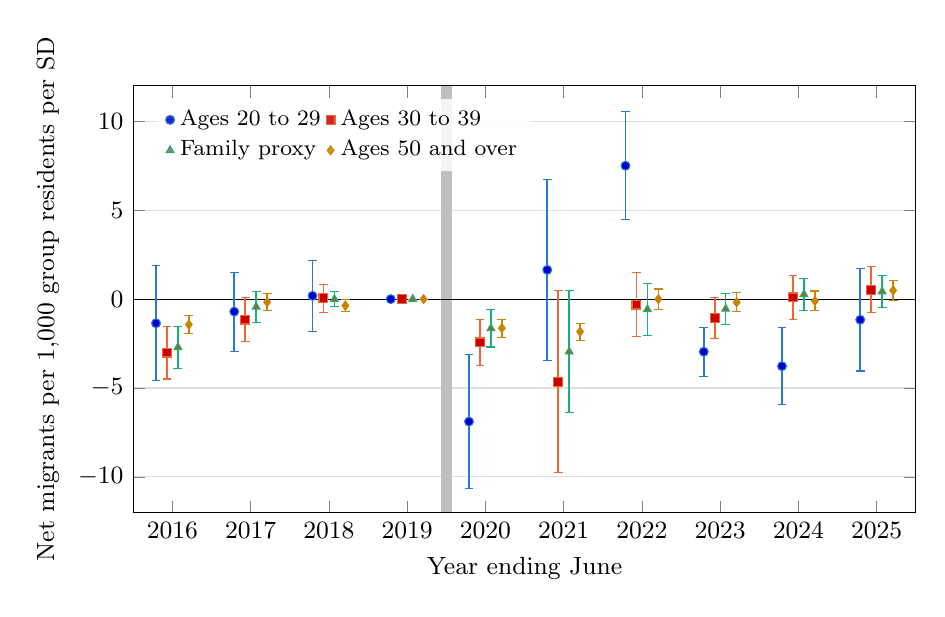
\begin{tikzpicture}
\begin{axis}[esaxis, height=7cm, xmin=2015.5, xmax=2025.5, ymin=-12, ymax=12, xtick={2016,...,2025},
  xlabel={Year ending June}, ylabel={Net migrants per 1,000 group residents per SD},
  legend pos=north west, legend columns=2]
\addplot[gray!50, line width=4pt, forget plot] coordinates {(2019.5,-12) (2019.5,12)};
\addplot[black, thin, forget plot] coordinates {(2015.5,0) (2025.5,0)};
\addplot+[ci, color=cA, mark=*] coordinates {(2015.79,-1.3552) +- (0,3.2259) (2016.79,-0.7027) +- (0,2.2198) (2017.79,0.1866) +- (0,1.9889) (2018.79,0.0000) +- (0,0.0000) (2019.79,-6.8895) +- (0,3.7789) (2020.79,1.6433) +- (0,5.0786) (2021.79,7.5036) +- (0,3.0479) (2022.79,-2.9601) +- (0,1.3875) (2023.79,-3.7724) +- (0,2.1520) (2024.79,-1.1601) +- (0,2.8855)};
\addlegendentry{Ages 20 to 29}
\addplot+[ci, color=cB, mark=square*] coordinates {(2015.93,-3.0081) +- (0,1.4824) (2016.93,-1.1491) +- (0,1.2166) (2017.93,0.0533) +- (0,0.7892) (2018.93,0.0000) +- (0,0.0000) (2019.93,-2.4356) +- (0,1.3011) (2020.93,-4.6465) +- (0,5.1135) (2021.93,-0.3038) +- (0,1.8015) (2022.93,-1.0612) +- (0,1.1726) (2023.93,0.0952) +- (0,1.2188) (2024.93,0.5256) +- (0,1.2949)};
\addlegendentry{Ages 30 to 39}
\addplot+[ci, color=cC, mark=triangle*] coordinates {(2016.07,-2.7096) +- (0,1.1775) (2017.07,-0.4398) +- (0,0.8782) (2018.07,-0.0042) +- (0,0.4330) (2019.07,0.0000) +- (0,0.0000) (2020.07,-1.6455) +- (0,1.0487) (2021.07,-2.9578) +- (0,3.4294) (2022.07,-0.5744) +- (0,1.4525) (2023.07,-0.5531) +- (0,0.8755) (2024.07,0.2635) +- (0,0.9068) (2025.07,0.4249) +- (0,0.9194)};
\addlegendentry{Family proxy}
\addplot+[ci, color=cD, mark=diamond*] coordinates {(2016.21,-1.4290) +- (0,0.4929) (2017.21,-0.1736) +- (0,0.4895) (2018.21,-0.3633) +- (0,0.3293) (2019.21,0.0000) +- (0,0.0000) (2020.21,-1.6317) +- (0,0.5038) (2021.21,-1.8316) +- (0,0.4804) (2022.21,-0.0012) +- (0,0.5723) (2023.21,-0.1810) +- (0,0.5381) (2024.21,-0.1020) +- (0,0.5582) (2025.21,0.4925) +- (0,0.5507)};
\addlegendentry{Ages 50 and over}
\end{axis}
\end{tikzpicture}
\caption{Net migration with the rest of the United Kingdom by age group and borough amenity density. Coefficients $\beta_k$ from equation~(\ref{eq:es}) with 95 per cent confidence intervals clustered by borough, offset horizontally. The family proxy combines ages 0 to 15 and 30 to 49. Thirty-two boroughs, 320 observations for each group.}\label{fig:age}
\end{figure}

Relative to older residents of the same borough and year, the net inflow of young adults fell during the closure and recovered at reopening (Figure~\ref{fig:ddd}, Table~\ref{tab:ddd}). Against the family proxy the coefficients are $-5.24$ in 2020, with a p-value of 0.002, $+4.60$ in 2021 and $+8.08$ in 2022, and the contrast $\theta_{2022} - \theta_{2020}$ is 13.32 with a p-value below 0.001. Against residents aged 50 and over the coefficients are $-5.26$, $+3.47$ and $+7.50$, with a contrast of 12.76. The coefficients for 2016 to 2018 lie between $-0.53$ and $+1.35$, with p-values of 0.34 or above, and the relative outflow resumed in 2023 and 2024, at $-2.41$ and $-4.04$ against the family proxy, during a period of higher interest rates and rising central rents.

\begin{figure}[htbp]
\centering
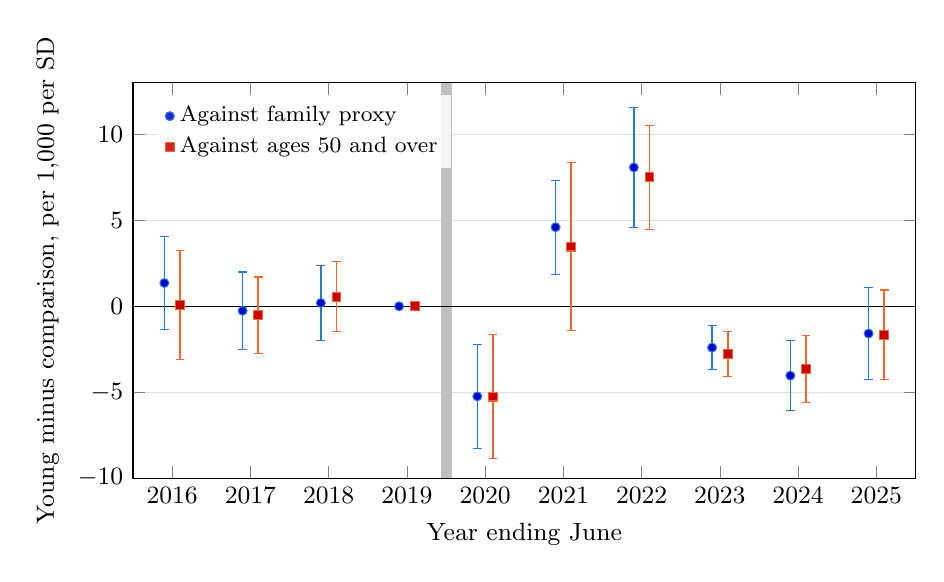
\begin{tikzpicture}
\begin{axis}[esaxis, height=6.6cm, xmin=2015.5, xmax=2025.5, ymin=-10, ymax=13, xtick={2016,...,2025},
  xlabel={Year ending June}, ylabel={Young minus comparison, per 1,000 per SD}, legend pos=north west]
\addplot[gray!50, line width=4pt, forget plot] coordinates {(2019.5,-10) (2019.5,13)};
\addplot[black, thin, forget plot] coordinates {(2015.5,0) (2025.5,0)};
\addplot+[ci, color=cA, mark=*] coordinates {(2015.9,1.3543) +- (0,2.7311) (2016.9,-0.2629) +- (0,2.2555) (2017.9,0.1907) +- (0,2.1706) (2018.9,0.0000) +- (0,0.0000) (2019.9,-5.2440) +- (0,3.0289) (2020.9,4.6011) +- (0,2.7411) (2021.9,8.0780) +- (0,3.5021) (2022.9,-2.4070) +- (0,1.2632) (2023.9,-4.0359) +- (0,2.0229) (2024.9,-1.5850) +- (0,2.7002)};
\addlegendentry{Against family proxy}
\addplot+[ci, color=cB, mark=square*] coordinates {(2016.1,0.0738) +- (0,3.1724) (2017.1,-0.5291) +- (0,2.2353) (2018.1,0.5498) +- (0,2.0314) (2019.1,0.0000) +- (0,0.0000) (2020.1,-5.2578) +- (0,3.5966) (2021.1,3.4749) +- (0,4.9033) (2022.1,7.5048) +- (0,3.0131) (2023.1,-2.7792) +- (0,1.3108) (2024.1,-3.6704) +- (0,1.9462) (2025.1,-1.6526) +- (0,2.6021)};
\addlegendentry{Against ages 50 and over}
\end{axis}
\end{tikzpicture}
\caption{Triple-difference coefficients $\theta_k$ from equation~(\ref{eq:ddd}) for London, with 95 per cent confidence intervals clustered by borough. Thirty-two boroughs, two groups and ten years, 640 observations for each comparison.}\label{fig:ddd}
\end{figure}

\begin{table}[htbp]
\centering
\caption{Triple difference, young adults against older residents of the same borough}\label{tab:ddd}
\small
\begin{tabularx}{\linewidth}{@{}L*{8}{c}@{}}
\toprule
\multicolumn{9}{@{}l}{\textit{Panel A. Yearly coefficients, year ending June (2019 omitted)}} \\
 & 2016 & 2017 & 2018 & 2020 & 2021 & 2022 & 2023 & 2024 \\
\midrule
Family proxy & $1.35$ & $-0.26$ & $0.19$ & $-5.24$ & $4.60$ & $8.08$ & $-2.41$ & $-4.04$ \\
 & ($0.341$) & ($0.819$) & ($0.881$) & ($0.002$) & ($0.014$) & ($<0.001$) & ($0.021$) & ($0.001$) \\[3pt]
Ages 50 and over & $0.07$ & $-0.53$ & $0.55$ & $-5.26$ & $3.47$ & $7.50$ & $-2.78$ & $-3.67$ \\
 & ($0.963$) & ($0.645$) & ($0.640$) & ($0.002$) & ($0.426$) & ($<0.001$) & ($0.020$) & ($0.003$) \\[3pt]
\bottomrule
\end{tabularx}

\medskip
\begin{tabularx}{\linewidth}{@{}L*{4}{c}@{}}
\toprule
\multicolumn{5}{@{}l}{\textit{Panel B. Period model (reference 2016 to 2019)}} \\
 & Closure & Reopening & Later & Reopening minus closure \\
\midrule
Family proxy & $-0.64$ & $7.76$ & $-3.00$ & $8.40$ \\
 & ($0.606$) & ($<0.001$) & ($0.001$) & ($<0.001$) \\[3pt]
Ages 50 and over & $-0.92$ & $7.48$ & $-2.72$ & $8.40$ \\
 & ($0.668$) & ($<0.001$) & ($0.027$) & ($<0.001$) \\[3pt]
\bottomrule
\end{tabularx}
\tabnote{Coefficients $\theta_k$ from equation~(\ref{eq:ddd}) per standard deviation of log amenity density, in net moves per 1,000 group residents, with wild cluster bootstrap p-values in brackets beneath (32 borough clusters). Years to June 2016 to 2025. In Panel B, closure is 2020 and 2021, reopening is 2022 and later is 2023 to 2025.}
\end{table}

\subsection{Robustness in London}\label{sec:robust}

The London reversal holds with controls for students and hospitality workers and among residents mostly past undergraduate age (Table~\ref{tab:robust}). The year to June 2022 contains the autumn term of 2021, and the 2011 student share correlates at 0.43 with amenity density, so with the student share interacted with year the contrast falls to 10.61 against the family proxy, with a p-value of 0.005, and with the five boroughs of highest student share removed it is 12.19, with a p-value of 0.004. Among 25 to 29 year olds the 2020 coefficient of $-5.25$ matches that of the full band and the 2022 coefficient of $+2.63$ is smaller, with a contrast of 7.87 and a p-value below 0.001, and against a linear trend through the 2016 to 2019 coefficients the 2022 coefficient lies 5.21 above trend against the family proxy, with a p-value of 0.004, and 2.92 above trend against residents aged 50 and over, with a p-value of 0.173. The 2011 hospitality share of employment among residents aged 16 to 34 correlates at 0.08 with amenity density, and with this share interacted with year the 2020 and 2022 coefficients move by less than 0.3 per 1,000.

\begin{table}[htbp]
\centering
\caption{Robustness of the young-adult response, London}\label{tab:robust}
\small
\begin{tabularx}{\linewidth}{@{}Lcccc@{}}
\toprule
 & 2020 & 2022 & Reopening minus closure & N \\
\midrule
\multicolumn{5}{@{}l}{\textit{Event studies}} \\
(1) Ages 20 to 29 & $-6.89$ & $7.50$ & $10.13$ & 320 \\
 & ($0.002$) & ($0.005$) & ($<0.001$)  & \\[3pt]
(2) Ages 20 to 29, students & $-6.83$ & $4.59$ & $7.31$ & 320 \\
 & ($0.009$) & ($0.048$) & ($0.003$)  & \\[3pt]
(3) Ages 20 to 29, drop five & $-7.42$ & $6.09$ & $8.53$ & 270 \\
 & ($0.013$) & ($0.070$) & ($0.003$)  & \\[3pt]
(4) Ages 20 to 29, hospitality & $-6.69$ & $7.47$ & $9.84$ & 320 \\
 & ($0.002$) & ($0.010$) & ($<0.001$)  & \\[3pt]
(5) Ages 20 to 24 & $-7.04$ & $14.06$ & $15.60$ & 320 \\
 & ($0.003$) & ($<0.001$) & ($<0.001$)  & \\[3pt]
(6) Ages 20 to 24, students & $-7.88$ & $9.13$ & $10.97$ & 320 \\
 & ($0.007$) & ($0.033$) & ($0.005$)  & \\[3pt]
(7) Ages 20 to 24, drop five & $-7.86$ & $11.49$ & $12.67$ & 270 \\
 & ($0.010$) & ($0.062$) & ($0.003$)  & \\[3pt]
(8) Ages 25 to 29 & $-6.89$ & $2.05$ & $5.63$ & 320 \\
 & ($0.002$) & ($0.131$) & ($0.002$)  & \\[3pt]
(9) Ages 25 to 29, students & $-6.14$ & $0.80$ & $4.29$ & 320 \\
 & ($0.008$) & ($0.491$) & ($0.010$)  & \\[3pt]
(10) Ages 25 to 29, drop five & $-7.14$ & $1.73$ & $5.20$ & 270 \\
 & ($0.013$) & ($0.395$) & ($0.019$)  & \\[3pt]
\multicolumn{5}{@{}l}{\textit{Triple differences}} \\
(11) Against family proxy & $-5.24$ & $8.08$ & $8.40$ & 640 \\
 & ($0.002$) & ($<0.001$) & ($<0.001$)  & \\[3pt]
(12) Against family proxy, hospitality & $-5.08$ & $8.03$ & $8.15$ & 640 \\
 & ($0.001$) & ($<0.001$) & ($<0.001$)  & \\[3pt]
(13) Against ages 50+ & $-5.26$ & $7.50$ & $8.40$ & 640 \\
 & ($0.002$) & ($<0.001$) & ($<0.001$)  & \\[3pt]
(14) Against ages 50+, hospitality & $-5.07$ & $7.45$ & $8.07$ & 640 \\
 & ($0.002$) & ($0.003$) & ($<0.001$)  & \\[3pt]
\bottomrule
\end{tabularx}
\tabnote{Coefficients per standard deviation of log amenity density, in net moves per 1,000 group residents, with wild cluster bootstrap p-values in brackets beneath. Years to June 2016 to 2025. Reopening minus closure is the 2022 coefficient minus the average of the 2020 and 2021 coefficients. In the students rows the 2011 full-time student share is interacted with year. In the drop-five rows Newham, Camden, Tower Hamlets, Southwark and Islington are removed, leaving 27 clusters. In the hospitality rows the 2011 share of employed residents aged 16 to 34 in accommodation, food or other services is interacted with year. Rows (11) to (14) are triple differences.}
\end{table}

Lower rents account for only part of the recovery. Rents in high-amenity boroughs followed their pre-2020 trend through the closure, and with each borough's change in log rent from 2019Q4 to 2021Q4 interacted with the young-adult indicator and year the contrast is 8.88 against the family proxy, with a p-value of 0.016, although that rent change correlates at $-0.76$ with amenity density, so much of the amenity variation itself is absorbed by the control. For moves between each borough and the other 31 the 2020 coefficient is $-2.04$ against the family proxy, against $-5.24$ for moves with the rest of the United Kingdom, so the outflow went mostly beyond the Greater London boundary, where the loss of variety is bundled with savings on rent for those moving to a parental home. Net international migration of young adults into high-amenity boroughs rose in 2020, with a coefficient of $+6.77$ against the family proxy, from a series modelled after the suspension of the International Passenger Survey and with 2016 coefficients of $+6.75$ to $+7.50$, so that series receives less weight than the internal one.

\subsection{Identification limits in London}\label{sec:idlim}

Within London the 2020 outflow cannot be separated from the response to teleworkability and garden access (Table~\ref{tab:idlim}). With teleworkability interacted with the young-adult indicator and year, the 2020 coefficient against the family proxy is $-1.18$, with a p-value of 0.595, and the contrast is 11.98, with a p-value of 0.010. With garden access the 2020 coefficient is $-3.22$, with a p-value of 0.090, and with both controls it is $+2.08$, with a contrast of 1.78 and p-values of 0.387 and 0.653, and the same pattern holds against residents aged 50 and over and for ages 25 to 29. Since amenity density correlates at 0.82 with teleworkability and at $-0.73$ with garden access across the 32 boroughs, only the combined response to central location, working from home and the lack of outdoor space can be identified across boroughs.

\begin{table}[htbp]
\centering
\caption{Teleworkability and garden access controls, London triple difference}\label{tab:idlim}
\small
\begin{tabularx}{\linewidth}{@{}L*{4}{c}@{}}
\toprule
 & 2020 & 2021 & 2022 & 2022 minus 2020 \\
\midrule
\multicolumn{5}{@{}l}{\textit{Ages 20 to 29 against the family proxy}} \\
No added control & $-5.24$ & $4.60$ & $8.08$ & $13.32$ \\
 & ($0.002$) & ($0.014$) & ($<0.001$) & ($<0.001$) \\[3pt]
Teleworkability & $-1.18$ & $4.13$ & $10.80$ & $11.98$ \\
 & ($0.595$) & ($0.154$) & ($0.001$) & ($0.010$) \\[3pt]
Garden access & $-3.22$ & $3.77$ & $2.28$ & $5.49$ \\
 & ($0.090$) & ($0.313$) & ($0.314$) & ($0.158$) \\[3pt]
Both & $2.08$ & $3.00$ & $3.86$ & $1.78$ \\
 & ($0.387$) & ($0.360$) & ($0.150$) & ($0.653$) \\[3pt]
\multicolumn{5}{@{}l}{\textit{Ages 20 to 29 against ages 50 and over}} \\
No added control & $-5.26$ & $3.47$ & $7.50$ & $12.76$ \\
 & ($0.002$) & ($0.426$) & ($<0.001$) & ($<0.001$) \\[3pt]
Teleworkability & $-0.29$ & $7.73$ & $12.07$ & $12.36$ \\
 & ($0.907$) & ($0.130$) & ($0.001$) & ($0.011$) \\[3pt]
Garden access & $-3.28$ & $3.40$ & $1.74$ & $5.03$ \\
 & ($0.165$) & ($0.510$) & ($0.401$) & ($0.176$) \\[3pt]
Both & $3.05$ & $8.34$ & $5.48$ & $2.43$ \\
 & ($0.330$) & ($0.297$) & ($0.002$) & ($0.570$) \\[3pt]
\multicolumn{5}{@{}l}{\textit{Ages 25 to 29 against the family proxy}} \\
No added control & $-5.25$ & $2.69$ & $2.63$ & $7.87$ \\
 & ($0.002$) & ($0.094$) & ($0.038$) & ($<0.001$) \\[3pt]
Teleworkability & $-2.72$ & $2.38$ & $3.07$ & $5.78$ \\
 & ($0.183$) & ($0.231$) & ($0.080$) & ($0.089$) \\[3pt]
Garden access & $-2.53$ & $0.51$ & $-0.37$ & $2.16$ \\
 & ($0.188$) & ($0.837$) & ($0.807$) & ($0.402$) \\[3pt]
Both & $1.17$ & $-0.45$ & $-0.68$ & $-1.85$ \\
 & ($0.620$) & ($0.801$) & ($0.595$) & ($0.559$) \\[3pt]
\multicolumn{5}{@{}l}{\textit{Ages 25 to 29 against ages 50 and over}} \\
No added control & $-5.26$ & $1.56$ & $2.05$ & $7.32$ \\
 & ($0.002$) & ($0.584$) & ($0.104$) & ($<0.001$) \\[3pt]
Teleworkability & $-1.83$ & $5.99$ & $4.33$ & $6.16$ \\
 & ($0.503$) & ($0.151$) & ($0.030$) & ($0.082$) \\[3pt]
Garden access & $-2.59$ & $0.13$ & $-0.90$ & $1.69$ \\
 & ($0.260$) & ($0.977$) & ($0.547$) & ($0.540$) \\[3pt]
Both & $2.14$ & $4.89$ & $0.94$ & $-1.20$ \\
 & ($0.573$) & ($0.395$) & ($0.440$) & ($0.720$) \\[3pt]
\bottomrule
\end{tabularx}
\tabnote{Coefficients $\theta_k$ from equation~(\ref{eq:ddd}) per standard deviation of log amenity density, in net moves per 1,000 group residents, with wild cluster bootstrap p-values in brackets beneath (32 borough clusters). Each control is standardised and interacted with the young-adult indicator and year. Years to June 2016 to 2025, 640 observations in each model.}
\end{table}

\subsection{The response to density across England and Wales}\label{sec:national}

Under its registered criterion, the national triple difference is evidence against the variety channel. Support was defined in the plan as a positive headline contrast with a p-value below 0.05 and a negative 2020 coefficient in specification (f), and evidence against as a contrast below zero or with a p-value of 0.10 or above in specification (f) together with a positive contrast in specification (a). In specification (f) the 2020 coefficient for ages 20 to 29 against the family proxy is $+1.82$, with a p-value of 0.030, and the contrast is $-1.53$, with a p-value of 0.191, while in specification (a) the contrast is $+3.12$, with a p-value of 0.113 (Table~\ref{tab:natreg}). The garden-access interaction for 2020 is $+4.34$, with a p-value below 0.001, whereby young adults moved towards districts with more private outdoor space relative to older residents, and under the plan the space and remote-working channel is partly supported. In a check chosen after the registered results, the contrast is $-0.94$ with the 2011 student share added and $-2.42$ with the 30 districts of highest student share excluded, with p-values of 0.415 and 0.060.

\begin{table}[htbp]
\centering
\caption{Registered national triple difference, England and Wales}\label{tab:natreg}
\footnotesize
\begin{tabularx}{\linewidth}{@{}L*{7}{c}@{}}
\toprule
 & 2016 & 2017 & 2018 & 2020 & 2021 & 2022 & 2022 minus 2020 \\
\midrule
\multicolumn{8}{@{}l}{\textit{Panel A. Ages 20 to 29 against the family proxy, 316 authorities}} \\
(a) No controls & $-1.05$ & $-0.14$ & $0.11$ & $-1.29$ & $1.55$ & $1.83$ & $3.12$ \\
 & ($0.187$) & ($0.899$) & ($0.877$) & ($0.183$) & ($0.306$) & ($0.160$) & ($0.113$) \\[3pt]
(b) Teleworkability & $-0.40$ & $0.27$ & $1.13$ & $0.59$ & $1.86$ & $2.63$ & $2.05$ \\
 & ($0.636$) & ($0.828$) & ($0.132$) & ($0.484$) & ($0.237$) & ($0.064$) & ($0.216$) \\[3pt]
(c) Garden access & $-0.91$ & $-0.77$ & $0.25$ & $2.12$ & $2.47$ & $-0.48$ & $-2.60$ \\
 & ($0.352$) & ($0.541$) & ($0.764$) & ($0.017$) & ($0.107$) & ($0.671$) & ($0.034$) \\[3pt]
(d) Both & $-0.65$ & $-0.50$ & $0.66$ & $2.41$ & $2.47$ & $0.20$ & $-2.20$ \\
 & ($0.491$) & ($0.701$) & ($0.436$) & ($0.006$) & ($0.114$) & ($0.855$) & ($0.078$) \\[3pt]
(e) Region by year & $-0.96$ & $0.23$ & $0.47$ & $-0.32$ & $2.03$ & $1.59$ & $1.91$ \\
 & ($0.228$) & ($0.819$) & ($0.509$) & ($0.650$) & ($0.185$) & ($0.156$) & ($0.155$) \\[3pt]
(f) Both and region by year & $-0.79$ & $-1.36$ & $0.04$ & $1.82$ & $2.63$ & $0.30$ & $-1.53$ \\
 & ($0.400$) & ($0.313$) & ($0.964$) & ($0.030$) & ($0.093$) & ($0.785$) & ($0.191$) \\[3pt]
\bottomrule
\end{tabularx}

\medskip
\begin{tabularx}{\linewidth}{@{}L*{5}{c}@{}}
\toprule
 & 2020 & 2022 & 2022 minus 2020 & Telework $\times$ 2020 & Garden $\times$ 2020 \\
\midrule
\multicolumn{6}{@{}l}{\textit{Panel B. Specification (f), other groups and samples}} \\
20 to 29 vs 50+ (316) & $1.70$ & $0.45$ & $-1.25$ & $-1.21$ & $3.32$ \\
 & ($0.048$) & ($0.723$) & ($0.306$) & ($0.259$) & ($0.002$) \\[3pt]
25 to 29 vs family (316) & $2.64$ & $0.96$ & $-1.68$ & $0.06$ & $5.08$ \\
 & ($0.001$) & ($0.184$) & ($0.087$) & ($0.955$) & ($<0.001$) \\[3pt]
25 to 29 vs 50+ (316) & $2.52$ & $1.11$ & $-1.41$ & $0.27$ & $4.05$ \\
 & ($0.003$) & ($0.195$) & ($0.186$) & ($0.822$) & ($<0.001$) \\[3pt]
20 to 29 vs family (284) & $2.88$ & $-0.91$ & $-3.79$ & $-0.55$ & $3.81$ \\
 & ($0.005$) & ($0.487$) & ($0.005$) & ($0.640$) & ($0.013$) \\[3pt]
20 to 29 vs 50+ (284) & $2.53$ & $-1.10$ & $-3.63$ & $-0.33$ & $2.86$ \\
 & ($0.013$) & ($0.436$) & ($0.010$) & ($0.787$) & ($0.070$) \\[3pt]
25 to 29 vs family (284) & $4.15$ & $0.54$ & $-3.61$ & $1.37$ & $5.10$ \\
 & ($<0.001$) & ($0.526$) & ($0.001$) & ($0.239$) & ($<0.001$) \\[3pt]
25 to 29 vs 50+ (284) & $3.80$ & $0.35$ & $-3.46$ & $1.59$ & $4.16$ \\
 & ($<0.001$) & ($0.731$) & ($0.004$) & ($0.218$) & ($0.005$) \\[3pt]
\bottomrule
\end{tabularx}
\tabnote{Coefficients $\theta_k$ from equation~(\ref{eq:ddd}) per standard deviation of the registered measure, log hospitality and leisure units per 1,000 residents, in net moves per 1,000 group residents, with wild cluster bootstrap p-values in brackets beneath, clustered by district. Years to June 2016 to 2025, 2019 omitted. Specification (f) is the registered headline. 316 districts, or 284 outside London.}
\end{table}

Tourist areas rank among the densest districts on the registered measure, because visitors raise the number of venues per resident. Outside the inner London boroughs the highest values belong to the Cotswolds, the Derbyshire Dales, South Hams, Gwynedd, Pembrokeshire and Stratford-on-Avon, while inner London, Manchester, Brighton and Hove and Bristol rank highest on the density and access measures. In Business Counts, 1,845 local units of racehorse owners are recorded in North Northamptonshire in 2019, against 15 in 2017, and these units are excluded from the measures chosen after the registered results.

With access to food venues as the measure, chosen after the registered results, young adults left dense districts in 2020 and returned by 2022 with teleworkability and garden access held fixed (Table~\ref{tab:measures}, Figure~\ref{fig:national}). The 2020 coefficient is $-5.54$ and the 2022 coefficient $+5.60$, the contrast is 11.14 with a p-value below 0.001, and outside London the contrast is 10.59. The contrast is 8.70 with density of venues per square kilometre, measure (b), and $-0.85$ with venues per resident, measure (a). With the access and density measures the coefficients for 2016 to 2018 are positive, at about 4 to 7, and against a linear trend through the pre-period the 2020 coefficient for measure (c) lies 5.28 below trend and the 2022 coefficient 9.36 above it, both with p-values below 0.001. From 2023 the coefficient is negative again, at $-4.69$ to $-9.94$, so the return of 2022 lasted one year.

\begin{table}[htbp]
\centering
\caption{Measures of density in the national triple difference}\label{tab:measures}
\small
\begin{tabularx}{\linewidth}{@{}L*{5}{c}@{}}
\toprule
 & 2020 & 2021 & 2022 & 2022 minus 2020 & Garden $\times$ 2020 \\
\midrule
\multicolumn{6}{@{}l}{\textit{316 authorities}} \\
Registered measure, units per resident & $1.82$ & $2.63$ & $0.30$ & $-1.53$ & $4.34$ \\
 & ($0.030$) & ($0.093$) & ($0.785$) & ($0.191$) & ($<0.001$) \\[3pt]
(a) Food, drink, arts and leisure per resident & $1.59$ & $2.88$ & $0.75$ & $-0.85$ & $4.26$ \\
 & ($0.067$) & ($0.112$) & ($0.521$) & ($0.502$) & ($<0.001$) \\[3pt]
(b) Food, drink, arts and leisure per km$^2$ & $-4.06$ & $-1.89$ & $4.64$ & $8.70$ & $1.81$ \\
 & ($<0.001$) & ($0.216$) & ($0.002$) & ($<0.001$) & ($0.061$) \\[3pt]
(c) Population-weighted access to food venues & $-5.54$ & $-3.85$ & $5.60$ & $11.14$ & $0.76$ \\
 & ($<0.001$) & ($0.046$) & ($0.001$) & ($<0.001$) & ($0.468$) \\[3pt]
\multicolumn{6}{@{}l}{\textit{284 authorities outside London}} \\
Registered measure, units per resident & $2.88$ & $1.04$ & $-0.91$ & $-3.79$ & $3.81$ \\
 & ($0.005$) & ($0.430$) & ($0.487$) & ($0.005$) & ($0.013$) \\[3pt]
(a) Food, drink, arts and leisure per resident & $3.00$ & $0.84$ & $-0.69$ & $-3.69$ & $3.86$ \\
 & ($0.009$) & ($0.577$) & ($0.645$) & ($0.017$) & ($0.011$) \\[3pt]
(b) Food, drink, arts and leisure per km$^2$ & $-3.91$ & $-1.62$ & $4.50$ & $8.42$ & $0.81$ \\
 & ($<0.001$) & ($0.285$) & ($0.001$) & ($<0.001$) & ($0.579$) \\[3pt]
(c) Population-weighted access to food venues & $-5.19$ & $-3.83$ & $5.40$ & $10.59$ & $-0.13$ \\
 & ($<0.001$) & ($0.046$) & ($0.002$) & ($<0.001$) & ($0.936$) \\[3pt]
\bottomrule
\end{tabularx}
\tabnote{Specification (f) of Table~\ref{tab:natreg} with each measure in place of the registered measure, ages 20 to 29 against the family proxy, with wild cluster bootstrap p-values in brackets beneath, clustered by district. SIC subclass 93191 is excluded from measures (a) and (b). Measures (a) to (c) were chosen after the registered results were known.}
\end{table}

\begin{figure}[htbp]
\centering
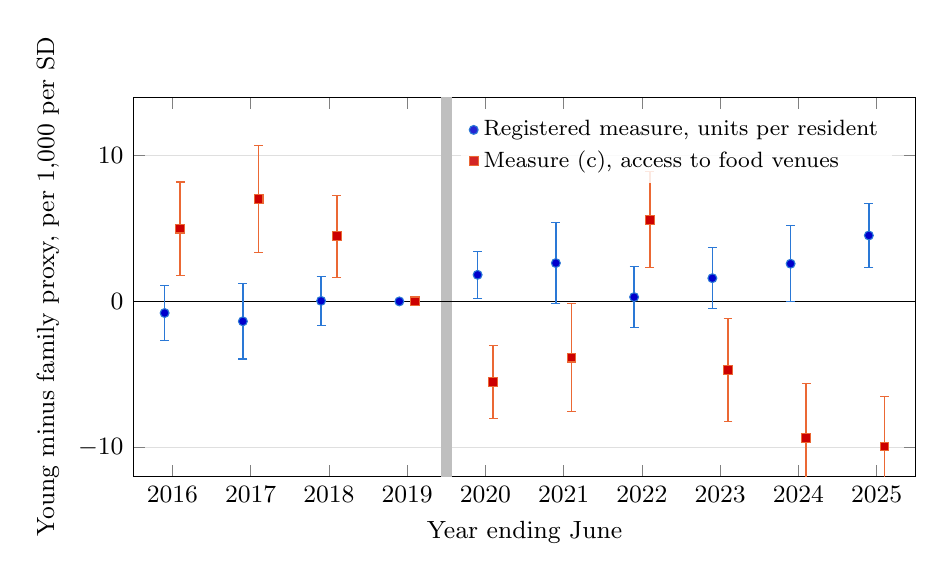
\begin{tikzpicture}
\begin{axis}[esaxis, height=6.4cm, xmin=2015.5, xmax=2025.5, ymin=-12, ymax=14, xtick={2016,...,2025},
  xlabel={Year ending June}, ylabel={Young minus family proxy, per 1,000 per SD}, legend pos=north east]
\addplot[gray!50, line width=4pt, forget plot] coordinates {(2019.5,-12) (2019.5,14)};
\addplot[black, thin, forget plot] coordinates {(2015.5,0) (2025.5,0)};
\addplot+[ci, color=cA, mark=*] coordinates {(2015.9,-0.7944) +- (0,1.8926) (2016.9,-1.3634) +- (0,2.5829) (2017.9,0.0374) +- (0,1.6859) (2018.9,0.0000) +- (0,0.0000) (2019.9,1.8231) +- (0,1.6011) (2020.9,2.6285) +- (0,2.7787) (2021.9,0.2972) +- (0,2.0943) (2022.9,1.5926) +- (0,2.0864) (2023.9,2.5834) +- (0,2.5916) (2024.9,4.5190) +- (0,2.1843)};
\addlegendentry{Registered measure, units per resident}
\addplot+[ci, color=cB, mark=square*] coordinates {(2016.1,4.9908) +- (0,3.1896) (2017.1,7.0276) +- (0,3.6623) (2018.1,4.4729) +- (0,2.8067) (2019.1,0.0000) +- (0,0.0000) (2020.1,-5.5368) +- (0,2.4960) (2021.1,-3.8519) +- (0,3.7110) (2022.1,5.5983) +- (0,3.2780) (2023.1,-4.6938) +- (0,3.5221) (2024.1,-9.3528) +- (0,3.7004) (2025.1,-9.9436) +- (0,3.4052)};
\addlegendentry{Measure (c), access to food venues}
\end{axis}
\end{tikzpicture}
\caption{National triple-difference coefficients for ages 20 to 29 against the family proxy, specification (f), with 95 per cent confidence intervals clustered by district. 316 districts. Measure (c) was chosen after the registered results were known.}\label{fig:national}
\end{figure}

Access to food venues correlates at 0.90 with log job density and at 0.89 with log population density, so the response to access is a response to density itself. With both densities interacted with the young-adult indicator and year, in a specification chosen after the registered results, the 2020 coefficient across all districts is $-5.47$, with a p-value of 0.024, and the contrast is 10.61, with a p-value below 0.001 (Table~\ref{tab:dens}). Outside London the 2020 coefficient is $-3.98$, with a p-value of 0.126, and with densities held fixed and a linear pre-trend removed the 2020 and 2022 deviations have p-values of 0.10 and 0.16. The value young adults place on dense locations is therefore identified beyond living space and remote working, and its consumption component is close to inseparable from the other benefits of density.

\begin{table}[htbp]
\centering
\caption{Access to food venues with density controls}\label{tab:dens}
\small
\begin{tabularx}{\linewidth}{@{}L*{4}{c}@{}}
\toprule
 & 2020 & 2021 & 2022 & 2022 minus 2020 \\
\midrule
\multicolumn{5}{@{}l}{\textit{Ages 20 to 29, 316 authorities}} \\
No density control & $-5.54$ & $-3.85$ & $5.60$ & $11.14$ \\
 & ($<0.001$) & ($0.046$) & ($0.001$) & ($<0.001$) \\[3pt]
Job density & $-5.31$ & $-7.64$ & $4.77$ & $10.08$ \\
 & ($0.023$) & ($0.021$) & ($0.066$) & ($<0.001$) \\[3pt]
Population density & $-5.58$ & $-6.10$ & $5.43$ & $11.01$ \\
 & ($0.021$) & ($0.089$) & ($0.042$) & ($<0.001$) \\[3pt]
Both densities & $-5.47$ & $-6.86$ & $5.14$ & $10.61$ \\
 & ($0.024$) & ($0.047$) & ($0.052$) & ($<0.001$) \\[3pt]
\multicolumn{5}{@{}l}{\textit{Ages 25 to 29, 316 authorities}} \\
No density control & $-5.34$ & $-2.07$ & $0.13$ & $5.46$ \\
 & ($<0.001$) & ($0.194$) & ($0.916$) & ($<0.001$) \\[3pt]
Job density & $-4.33$ & $-0.40$ & $0.63$ & $4.95$ \\
 & ($0.037$) & ($0.882$) & ($0.791$) & ($0.062$) \\[3pt]
Population density & $-4.97$ & $0.46$ & $-0.43$ & $4.54$ \\
 & ($0.019$) & ($0.866$) & ($0.855$) & ($0.085$) \\[3pt]
Both densities & $-4.68$ & $0.20$ & $0.00$ & $4.68$ \\
 & ($0.027$) & ($0.940$) & ($1.000$) & ($0.080$) \\[3pt]
\multicolumn{5}{@{}l}{\textit{Ages 20 to 29, 284 authorities outside London}} \\
No density control & $-5.19$ & $-3.83$ & $5.40$ & $10.59$ \\
 & ($<0.001$) & ($0.046$) & ($0.002$) & ($<0.001$) \\[3pt]
Job density & $-3.66$ & $-8.44$ & $4.17$ & $7.83$ \\
 & ($0.148$) & ($0.012$) & ($0.140$) & ($0.010$) \\[3pt]
Population density & $-4.15$ & $-9.33$ & $4.00$ & $8.15$ \\
 & ($0.111$) & ($0.007$) & ($0.168$) & ($0.007$) \\[3pt]
Both densities & $-3.98$ & $-9.20$ & $4.02$ & $7.99$ \\
 & ($0.126$) & ($0.008$) & ($0.165$) & ($0.008$) \\[3pt]
\multicolumn{5}{@{}l}{\textit{Ages 25 to 29, 284 authorities outside London}} \\
No density control & $-4.96$ & $-2.02$ & $-0.07$ & $4.89$ \\
 & ($<0.001$) & ($0.202$) & ($0.960$) & ($0.001$) \\[3pt]
Job density & $-2.58$ & $-0.97$ & $-0.21$ & $2.37$ \\
 & ($0.246$) & ($0.694$) & ($0.935$) & ($0.414$) \\[3pt]
Population density & $-3.39$ & $-1.66$ & $-1.84$ & $1.55$ \\
 & ($0.135$) & ($0.514$) & ($0.486$) & ($0.591$) \\[3pt]
Both densities & $-3.10$ & $-1.44$ & $-1.38$ & $1.72$ \\
 & ($0.167$) & ($0.566$) & ($0.596$) & ($0.556$) \\[3pt]
\bottomrule
\end{tabularx}
\tabnote{Specification (f) with measure (c) in place of the registered measure and with log job density, log population density or both, standardised and interacted with the young-adult indicator and year, against the family proxy. Wild cluster bootstrap p-values in brackets beneath, clustered by district. The measure and the density controls were chosen after the registered results were known.}
\end{table}

\subsection{Separating consumption variety}\label{sec:separate}

Consumption variety cannot be separated from the other benefits of density under any of the four designs, and each design falls short for a reason tied to its source of variation (Table~\ref{tab:designs}). In the London borough design the 2020 response is close to zero once teleworkability and garden access are controlled (Section~\ref{sec:idlim}), and in the registered national design tourist areas rank among the densest on the per-resident measure, while the access measures with which the London pattern reappears correlate at about 0.9 with job and population density (Section~\ref{sec:national}).

\begin{table}[htbp]
\centering
\caption{Four designs for separating consumption variety}\label{tab:designs}
\footnotesize
\begin{tabularx}{\linewidth}{@{}>{\raggedright\arraybackslash}p{2.1cm}>{\raggedright\arraybackslash}p{2.6cm}>{\raggedright\arraybackslash}p{1.9cm}>{\raggedright\arraybackslash}p{2.6cm}L@{}}
\toprule
Design & Separating variation & Registration & Headline (p-value) & Shortfall \\
\midrule
London boroughs & Amenity density with teleworkability and garden controls, 32 boroughs & None & 2020 coefficient $+2.08$ (0.387) with both controls & Amenity density correlates at 0.82 and $-0.73$ with the controls \\
National triple difference & Venues per resident, 316 districts & National plan & Contrast $-1.53$ (0.191) & Measure high in tourist areas; access measures correlate at about 0.9 with density \\
Tier closures & Extra closure days beyond national lockdowns, 316 districts & National plan & Interaction with density $+0.24$ (0.847) & Annual totals fail the cross-section first stage (0.581) \\
Venue mix & Variety-days lost within districts, 6,797 MSOAs & Venue-mix plan & $-1.28$ per 10 days (0.011) & Placebo $+3.28$ ($<0.001$) fails the registered rule \\
\bottomrule
\end{tabularx}
\tabnote{Wild cluster bootstrap p-values. The London contrast is for ages 20 to 29 against the family proxy, the national designs are for ages 20 to 29 against the family proxy, and the venue-mix headline is for Census inflow rates at ages 25 to 34.}
\end{table}

Under its registered criterion the tier design is uninformative, and its outcome coefficient is evidence against the variety channel. In the plan the design was to be treated as uninformative if its first stage had a bootstrap p-value of 0.10 or above, and an interaction coefficient at or above zero, or with a p-value of 0.10 or above, was to count against variety. Extra days of indoor hospitality closure in the year to June 2021 average 21 per district, with a maximum of 65 in Leicester, and within districts Google retail and recreation visits fell by 1.13 percentage points per ten extra days, while across districts the annual total has a first-stage coefficient of 0.20 with a p-value of 0.581. The interaction of extra closure days with amenity density is $+0.24$, with a p-value of 0.847, and extra days were set mainly by case rates, at 0.48 standard deviations per standard deviation.

The venue-mix design is built on a closure calendar coded from the regulations for seven venue types (Table~\ref{tab:calendar}). Forty-two rules were coded from legislation.gov.uk, each checked against the text of the regulation, with a value of 1 for closure to the public, 0.5 for partial closure such as outdoor service only and 0 for opening, and only legal requirements were coded, so English theatres count as open from 4 July 2020 although guidance advised against indoor performances until 15 August. Takeaways never closed, nightclubs were closed throughout the main window, and theatres in Wales were closed from March 2020 to May 2021 without a break. Restaurants and cafes form 52 per cent of access, takeaways 26 per cent and pubs and bars 20 per cent, while cinemas, theatres, gyms and nightclubs together form about 2 per cent, so variety-days lost correlates at $-0.92$ with the takeaway share of access and behaves almost as an inverse takeaway share.

\begin{table}[htbp]
\centering
\caption{Closure calendar by venue type}\label{tab:calendar}
\small
\begin{tabularx}{\linewidth}{@{}Lccccc@{}}
\toprule
 & \multicolumn{2}{c}{23 Mar 2020 to 22 Mar 2021} & \multicolumn{2}{c}{1 Apr to 31 Jul 2021} & Share of \\
 & England & Wales & England & Wales & access, \% \\
\midrule
Pubs and bars & 0.65 (0.56--0.74) & 0.66 & 0.23 & 0.29 & 20 \\
Restaurants and cafes & 0.63 (0.56--0.74) & 0.64 & 0.23 & 0.29 & 52 \\
Takeaways & 0 & 0 & 0 & 0 & 26 \\
Cinemas & 0.63 (0.56--0.74) & 0.69 & 0.38 & 0.38 & 0.3 \\
Theatres and concert venues & 0.63 (0.56--0.74) & 1.00 & 0.38 & 0.38 & 0.6 \\
Gyms & 0.65 (0.62--0.76) & 0.69 & 0.09 & 0.26 & 0.6 \\
Nightclubs & 1.00 & 1.00 & 0.89 & 1.00 & 0.4 \\
\bottomrule
\end{tabularx}
\tabnote{Shares of days closed, with 0.5 for partial closure. English values are means over districts with ranges in brackets, and the April to July 2021 shares are the same in every English district. Shares of access are means over MSOAs of the access index at a decay of 1.5 km. Arts centres are counted with theatres.}
\end{table}

The stopping rule of the venue-mix design was applied before any outcome was opened, and the residual variation of the treatment lay well above its threshold. Variety-days lost has a mean of 171 days and a standard deviation of 17.9 across 6,856 English MSOAs, district fixed effects and the nine controls explain 67 per cent of its variance, and the residual standard deviation is 10.4 days, or 58 per cent of the raw standard deviation, against a stopping threshold of 2 days or 10 per cent. Within districts the treatment correlates at 0.41 with teleworkability and at $-0.33$ with log population density. The plan was then written and fixed by its checksum.

Under the registered rule the verdict of the venue-mix design is that the variety channel is not supported (Table~\ref{tab:vm}). The headline coefficient for ages 25 to 34 is $-1.28$ per 10 days, or $-2.29$ per standard deviation, with a p-value of 0.011, so the first condition holds. The placebo on the 2001 to 2011 change is $+3.28$, with a p-value below 0.001, opposite in sign and more than twice the size of the headline, so the second condition fails. The coefficient for ages 50 and over is $+0.24$ and the stacked difference is $-0.19$, with a p-value of 0.743, so the third condition holds in sign. The pattern of a faster rise in young inflow rates from 2001 to 2011 followed by a slower rise from 2011 to 2021 is consistent with mean reversion at least as much as with the closures, and the same pattern of opposite signs arose in the Census design of the national plan, under which the support criterion was met with a coefficient of $-6.18$ per standard deviation of access at ages 20 to 34 and a placebo of $+3.74$, subject to a caveat about mean reversion.

\begin{table}[htbp]
\centering
\caption{Venue-mix design, variety-days lost and young-adult inflow rates}\label{tab:vm}
\footnotesize
\begin{tabularx}{\linewidth}{@{}Lcccc@{}}
\toprule
 & Per 10 days & 95\% CI & p-value & Per SD \\
\midrule
\multicolumn{5}{@{}l}{\textit{Panel A. Registered decision rule, MSOAs, change from Census 2011 to Census 2021}} \\
(1) Headline, ages 25 to 34 & $-1.28$ & [$-2.25$, $-0.31$] & $0.011$ & $-2.29$ \\
(2) Placebo, change from 2001 to 2011, ages 25 to 34 & $3.28$ & [$2.27$, $4.29$] & $<0.001$ & $5.88$ \\
(3) Ages 50 and over & $0.24$ & [$-0.06$, $0.55$] & $0.116$ & $0.44$ \\
(4) Stacked, ages 25 to 34 minus 50 and over & $-0.19$ & [$-1.29$, $0.90$] & $0.743$ & $-0.34$ \\
\midrule
\multicolumn{5}{@{}l}{\textit{Panel B. Further registered estimates, outside the decision rule}} \\
(5) Ages 20 to 24 & $-2.08$ & [$-3.54$, $-0.62$] & $0.006$ & $-3.72$ \\
(6) Ages 20 to 34 & $-1.46$ & [$-2.42$, $-0.51$] & $0.004$ & $-2.62$ \\
(7) District effects only & $0.65$ & [$-0.29$, $1.59$] & $0.173$ & $1.17$ \\
(8) District effects and teleworkability only & $-1.97$ & [$-2.99$, $-0.96$] & $<0.001$ & $-3.53$ \\
(9) District effects and garden access only & $1.03$ & [$0.13$, $1.93$] & $0.024$ & $1.84$ \\
(10) Top decile of student share dropped & $-1.02$ & [$-1.95$, $-0.10$] & $0.034$ & $-1.81$ \\
(11) OpenStreetMap 2019 venues & $-0.96$ & [$-1.59$, $-0.33$] & $0.004$ & $-2.19$ \\
(12) England and Wales & $-1.30$ & [$-2.22$, $-0.38$] & $0.007$ & $-2.34$ \\
(13) England outside London & $-1.37$ & [$-2.38$, $-0.35$] & $0.012$ & $-2.47$ \\
(14) Stacked, district-by-age effects & $-1.53$ & [$-2.51$, $-0.54$] & $0.004$ & $-2.73$ \\
(15) District panel, year to June 2021 & $-1.19$ & [$-3.88$, $1.50$] & $0.398$ & \\
(16) District panel, reopening test, 2022 minus 2021 & $-0.50$ & [$-9.39$, $8.38$] & $0.926$ & \\
\bottomrule
\end{tabularx}
\tabnote{Rows (1) to (14) are coefficients from equation~(\ref{eq:vm}) on the change in movers per 1,000 residents of the band between Censuses, with district fixed effects and the nine controls unless stated, 6,797 English MSOAs in 294 districts for the headline. Rows (15) and (16) are from the national triple difference with variety-days lost in place of the amenity measure, ages 20 to 29 against the family proxy, 316 districts. Confidence intervals from cluster-robust standard errors and wild cluster bootstrap p-values, clustered by district.}
\end{table}

The verdict is unchanged in the further registered estimates. The sign of the headline depends on the controls, at $+0.65$ with district effects alone, $-1.97$ with teleworkability alone and between $+1.03$ and $+1.32$ with garden access, flats or private renting alone. In the district panel the treatment for the year to June 2021 has a coefficient of $-1.19$ in that year, with a p-value of 0.398, and in the registered reopening test a smaller recovery where more variety stayed closed from April to July 2021 would give a negative contrast, estimated at $-0.50$ with a p-value of 0.926. The venue counts come from the hygiene register as held in 2026, so venues that closed after 2019 are missing, and the OpenStreetMap version for 2019 gives a similar headline of $-0.96$.

\subsection{Recovery after reopening}\label{sec:recovery}

Under the registered rule the recovery test is inconclusive (Table~\ref{tab:rec}, Figure~\ref{fig:rec}). The first stage has a coefficient of $-0.0082$ log points of shock per standard deviation of access, with a standard error of 0.0014 and a cluster-robust F of 33.0, so the Wald interval applies. The headline coefficient across 7,262 MSOAs in 316 districts at ages 25 to 34 is $-0.51$, with a 95 per cent interval from $-1.11$ to $0.10$ that contains both benchmarks. Against $-1$ the Wald p-value is 0.111 and the Anderson-Rubin bootstrap p-value is 0.178, against 0 they are 0.103 and 0.058, and the Anderson-Rubin set runs from $-1.31$ to $0.01$. The OLS coefficient is $+0.35$, so small areas whose young-adult population fell further from 2019 to 2021 kept falling, and the sign is reversed once the shock is instrumented.

\begin{figure}[htbp]
\centering
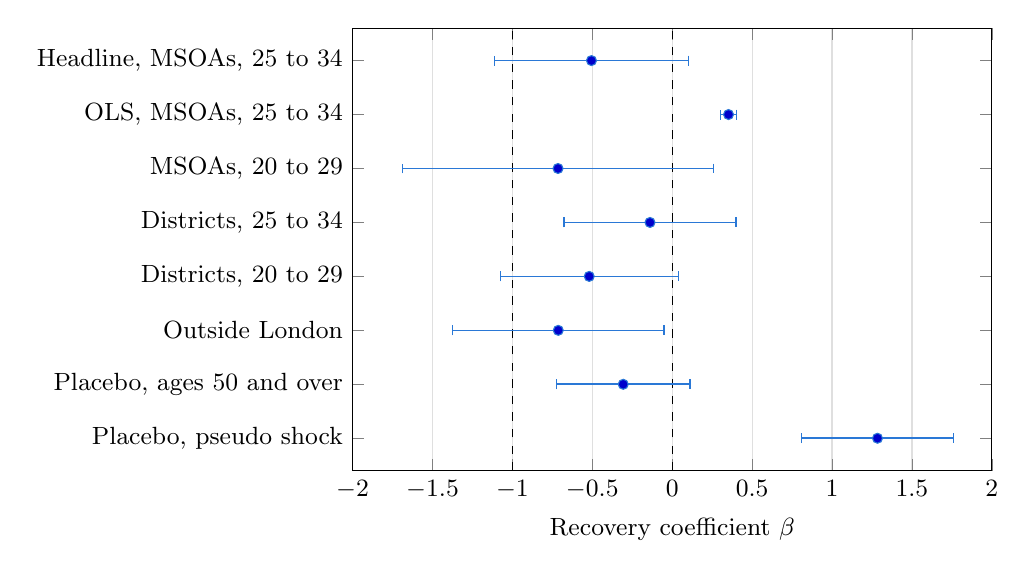
\begin{tikzpicture}
\begin{axis}[width=0.8\linewidth, height=7.2cm, xmin=-2, xmax=2, ymin=0.4, ymax=8.6,
  ytick={1,...,8}, yticklabels={{Placebo, pseudo shock},{Placebo, ages 50 and over},{Outside London},{Districts, 20 to 29},{Districts, 25 to 34},{MSOAs, 20 to 29},{OLS, MSOAs, 25 to 34},{Headline, MSOAs, 25 to 34}}, xmajorgrids, grid style={gray!25},
  tick label style={font=\small}, label style={font=\small},
  xlabel={Recovery coefficient $\beta$}]
\addplot[black, dashed, forget plot] coordinates {(-1,0.4) (-1,8.6)};
\addplot[black, dashed, forget plot] coordinates {(0,0.4) (0,8.6)};
\addplot+[only marks, color=cA, mark=*, mark size=1.8pt, error bars/x dir=both, error bars/x explicit,
  error bars/error bar style={line width=0.6pt}] coordinates {(-0.5053,8) +- (0.6087,0) (0.3523,7) +- (0.0488,0) (-0.7146,6) +- (0.9719,0) (-0.1390,5) +- (0.5381,0) (-0.5193,4) +- (0.5578,0) (-0.7130,3) +- (0.6614,0) (-0.3065,2) +- (0.4181,0) (1.2844,1) +- (0.4779,0)};
\end{axis}
\end{tikzpicture}
\caption{Recovery coefficients from equation~(\ref{eq:rec}) with 95 per cent Wald intervals clustered by district. Dashed lines are drawn at full recovery, $-1$, and at a lasting shift, 0. District rows are for recovery to 2025, with region fixed effects. The London estimate, with a first-stage F of 1.3 and an unbounded Anderson-Rubin set, is omitted.}\label{fig:rec}
\end{figure}

\begin{table}[htbp]
\centering
\caption{Recovery of young-adult populations, Davis and Weinstein coefficients}\label{tab:rec}
\footnotesize
\begin{tabularx}{\linewidth}{@{}Lrcr>{\centering\arraybackslash}p{3.3cm}>{\raggedright\arraybackslash}p{2.2cm}@{}}
\toprule
 & $\beta$ & 95\% CI & F & Anderson-Rubin set & Reading \\
\midrule
\multicolumn{6}{@{}l}{\textit{Panel A. Registered headline}} \\
(1) MSOAs, ages 25 to 34, measure (c) & $-0.51$ & [$-1.11$, $0.10$] & $33.0$ & [$-1.31$, $0.01$] & inconclusive \\
\midrule
\multicolumn{6}{@{}l}{\textit{Panel B. Further registered estimates}} \\
(2) MSOAs, 25 to 34, OLS & $0.35$ & [$0.30$, $0.40$] &  &  & shock deepened \\
(3) MSOAs, 25 to 34, variety-days lost & $0.56$ & [$-0.39$, $1.51$] & $8.9$ & [$-0.68$, $1.86$] & lasting shift \\
(4) MSOAs, 20 to 29, measure (c) & $-0.71$ & [$-1.69$, $0.26$] & $15.3$ & [$-2.46$, $0.01$] & inconclusive \\
(5) Districts, 25 to 34, to 2025 & $-0.14$ & [$-0.68$, $0.40$] & $82.1$ & [$-0.73$, $0.36$] & lasting shift \\
(6) Districts, 25 to 34, to 2024 & $-0.17$ & [$-0.63$, $0.29$] & $82.1$ & [$-0.69$, $0.26$] & lasting shift \\
(7) Districts, 25 to 34, variety-days lost & $-1.08$ & [$-2.72$, $0.56$] & $10.0$ & [$-4.49$, $0.20$] & inconclusive \\
(8) Districts, 20 to 29, to 2025 & $-0.52$ & [$-1.08$, $0.04$] & $45.5$ & [$-1.15$, $0.02$] & inconclusive \\
(9) Districts, 20 to 29, to 2024 & $-0.62$ & [$-1.11$, $-0.13$] & $45.5$ & [$-1.20$, $-0.17$] & full recovery \\
\midrule
\multicolumn{6}{@{}l}{\textit{Panel C. Registered heterogeneity, MSOAs, ages 25 to 34}} \\
(10) London & $0.15$ & [$-2.71$, $3.00$] & $1.3$ & unbounded & inconclusive, unbounded \\
(11) Rest of England and Wales & $-0.71$ & [$-1.37$, $-0.05$] & $27.9$ & [$-1.65$, $-0.17$] & full recovery \\
(12) Density, lowest tercile & $-2.28$ & [$-6.92$, $2.37$] & $1.7$ & ($-\infty$, $-0.14$] & inconclusive, unbounded \\
(13) Density, middle tercile & $-2.04$ & [$-4.14$, $0.06$] & $7.4$ & ($-\infty$, $-0.77$] & inconclusive, unbounded \\
(14) Density, highest tercile & $24.84$ & [$-80.43$, $130.11$] & $0.2$ & empty & inconclusive, empty set \\
(15) Access, lowest tercile & $-3.66$ & [$-14.78$, $7.46$] & $0.6$ & ($-\infty$, $-0.10$] $\cup$ [$2.64$, $+\infty$) & inconclusive, unbounded \\
(16) Access, middle tercile & $-0.46$ & [$-1.59$, $0.68$] & $6.9$ & [$-3.33$, $0.56$] & inconclusive \\
(17) Access, highest tercile & $13.06$ & [$-38.44$, $64.56$] & $0.2$ & ($-\infty$, $-2.41$] $\cup$ [$2.91$, $+\infty$) & inconclusive, unbounded \\
\midrule
\multicolumn{6}{@{}l}{\textit{Panel D. Registered placebos, MSOAs}} \\
(18) Ages 50 and over & $-0.31$ & [$-0.72$, $0.11$] & $55.8$ & [$-0.80$, $0.07$] & lasting shift \\
(19) Pseudo shock 2015 to 2017, ages 25 to 34 & $1.28$ & [$0.81$, $1.76$] & $28.8$ & [$0.88$, $1.93$] & shock deepened \\
\bottomrule
\end{tabularx}
\tabnote{Coefficients from equation~(\ref{eq:rec}), instrumented by measure (c) unless stated, with Wald intervals from standard errors clustered by district and the cluster-robust first-stage F. Readings are classified under the registered rule, with the Anderson-Rubin set where F is below 10, and the verdict rests on row (1) alone. MSOA models have district fixed effects and recovery to 2024, with 7,262 MSOAs in 316 districts in the full sample. District models have region fixed effects. The pseudo shock is the change from 2015 to 2017, with recovery from 2017 to 2019 and a trend from 2011 to 2015. The headline minus the pseudo coefficient is $-1.79$, with a 95 per cent interval from $-2.54$ to $-1.04$.}
\end{table}

The access instrument is undermined by the pseudo-shock placebo. With the shock set to the change from 2015 to 2017 and the recovery to the change from 2017 to 2019, the instrumented coefficient is $+1.28$, with an interval from 0.81 to 1.76 and a first-stage F of 28.8, so high-access MSOAs whose young-adult growth slowed in ordinary years kept slowing beyond their 2011 to 2015 trend. Access is therefore related to young-adult growth in periods without closures, and the exclusion restriction, under which access affects growth after 2021 only through the shock of 2019 to 2021, is doubtful. Recovery from the closures is therefore mixed in the headline with a dynamic already associated with access, and the coefficient for ages 50 and over is $-0.31$, with an interval from $-0.72$ to $0.11$, a reading of a lasting shift. The mid-2021 estimates at both levels rest on the census of March 2021, taken during the third lockdown.

Two secondary readings, both registered as further estimates outside the decision rule, are more favourable to recovery. Relative to ordinary momentum the recovery was large, since the headline minus the pseudo coefficient is $-1.79$, with an interval from $-2.54$ to $-1.04$, a reading that holds only if the dynamic carried by access from 2015 to 2019 would have continued unchanged after 2021. Outside London the coefficient is $-0.71$, with an interval from $-1.37$ to $-0.05$ and a first-stage F of 27.9, a reading of full recovery, while in London the first-stage F is 1.3 and the Anderson-Rubin set is unbounded, so whether the largest city persisted cannot be tested with this instrument. Five of the six terciles of density and access have first-stage F statistics below 10, and the Anderson-Rubin set for the densest tercile is empty. Across districts, where measure (c) is a strong instrument with an F of 82.1, the coefficient at ages 25 to 34 is $-0.14$, a reading of a lasting shift, while at ages 20 to 29 it is $-0.52$ to 2025 and $-0.62$ to 2024, the latter a reading of full recovery. Variety-days lost is a weak instrument, with F statistics from 1.2 to 10.0 and a first stage that changes sign between MSOAs and districts. These readings are suggestive evidence against a residential counterpart of the tipping that \citet{monte2026} find for commuting, with the limit that their result concerns the largest cities, where the present instrument is weakest.

\subsection{Prices}\label{sec:prices}

Prices in London moved with persistent channels, with little response specific to the closure. Rents in high-amenity boroughs fell by 0.20 log points a quarter relative to other boroughs before 2020, followed that trend through the closure, and from 2023Q3 to 2026Q3 lay 4.39 log points above it on average, with a p-value of 0.015, a recovery whose size depends on the trend assumption (Figure~\ref{fig:rent}). For house prices, with MSOA and borough-by-quarter fixed effects and distance to Charing Cross, teleworkability, garden access and property type interacted with quarter, the closure-window average is $-0.28$ log points per standard deviation of MSOA amenity density, with a 95 per cent confidence interval from $-1.78$ to $1.21$, and access to venues within 1.5 kilometres correlates at $-0.85$ with distance to Charing Cross within boroughs. Price-to-rent ratios in high-amenity Inner London fell from 113.8 in 2021Q4 to 74.5 in 2025Q4, against 102.0 and 88.4 in low-amenity Outer London, consistent with financing costs bearing most heavily on high-priced central housing. Across England and Wales the average deviation of high-amenity rents from their projected trend over 2020Q2 to 2021Q2 is $+0.15$ log points, with a p-value of 0.569, under the registered rent design.

\begin{figure}[htbp]
\centering
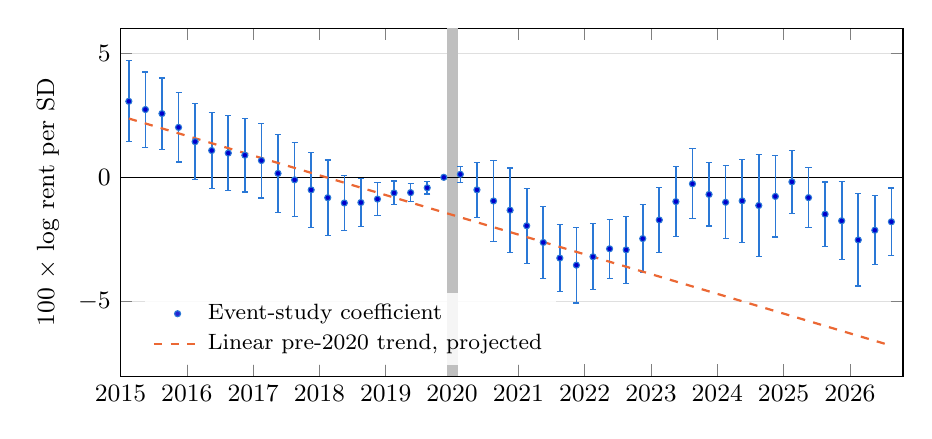
\begin{tikzpicture}
\begin{axis}[esaxis, height=6cm, xmin=2015, xmax=2026.8, ymin=-8, ymax=6, xtick={2015,...,2026},
  ylabel={100 $\times$ log rent per SD}, legend pos=south west]
\addplot[gray!50, line width=4pt, forget plot] coordinates {(2020,-8) (2020,6)};
\addplot[black, thin, forget plot] coordinates {(2015,0) (2026.8,0)};
\addplot+[ci, color=cA, mark=*, mark size=1.1pt] coordinates {(2015.125,3.0588) +- (0,1.6315) (2015.375,2.7281) +- (0,1.5127) (2015.625,2.5656) +- (0,1.4303) (2015.875,2.0108) +- (0,1.3931) (2016.125,1.4357) +- (0,1.5305) (2016.375,1.0797) +- (0,1.5253) (2016.625,0.9749) +- (0,1.5114) (2016.875,0.8902) +- (0,1.4796) (2017.125,0.6766) +- (0,1.5074) (2017.375,0.1582) +- (0,1.5756) (2017.625,-0.1013) +- (0,1.4878) (2017.875,-0.5053) +- (0,1.5221) (2018.125,-0.8196) +- (0,1.5155) (2018.375,-1.0323) +- (0,1.1184) (2018.625,-1.0133) +- (0,0.9572) (2018.875,-0.8751) +- (0,0.6626) (2019.125,-0.6272) +- (0,0.4786) (2019.375,-0.6155) +- (0,0.3566) (2019.625,-0.4215) +- (0,0.2505) (2019.875,0.0000) +- (0,0.0000) (2020.125,0.1213) +- (0,0.3283) (2020.375,-0.5049) +- (0,1.0973) (2020.625,-0.9512) +- (0,1.6242) (2020.875,-1.3224) +- (0,1.6972) (2021.125,-1.9499) +- (0,1.5040) (2021.375,-2.6203) +- (0,1.4387) (2021.625,-3.2490) +- (0,1.3342) (2021.875,-3.5334) +- (0,1.5234) (2022.125,-3.1953) +- (0,1.3249) (2022.375,-2.8758) +- (0,1.1901) (2022.625,-2.9188) +- (0,1.3517) (2022.875,-2.4659) +- (0,1.3808) (2023.125,-1.7167) +- (0,1.2924) (2023.375,-0.9762) +- (0,1.3981) (2023.625,-0.2601) +- (0,1.4082) (2023.875,-0.6884) +- (0,1.2687) (2024.125,-1.0038) +- (0,1.4719) (2024.375,-0.9465) +- (0,1.6735) (2024.625,-1.1331) +- (0,2.0597) (2024.875,-0.7682) +- (0,1.6327) (2025.125,-0.1836) +- (0,1.2597) (2025.375,-0.8172) +- (0,1.2179) (2025.625,-1.4820) +- (0,1.2923) (2025.875,-1.7482) +- (0,1.5644) (2026.125,-2.5201) +- (0,1.8537) (2026.375,-2.1289) +- (0,1.3851) (2026.625,-1.7882) +- (0,1.3570)};
\addlegendentry{Event-study coefficient}
\addplot[cB, thick, dashed] coordinates {(2015.125,2.3665) (2026.625,-6.7758)};
\addlegendentry{Linear pre-2020 trend, projected}
\end{axis}
\end{tikzpicture}
\caption{Private rents by borough amenity density. Quarterly event-study coefficients relative to 2019Q4, with the linear trend fitted to 2015Q1 to 2019Q4 and projected forward (slope -0.20 per quarter, level -1.41 at 2019Q4). Confidence intervals at 95 per cent, clustered by borough; 32 boroughs, 1,504 observations. Values for 2026 are provisional.}\label{fig:rent}
\end{figure}

%======================================================================
\section{Conclusion}\label{sec:conclusion}
%======================================================================

The COVID-19 closures temporarily removed much of the residential value of dense places and restored it on known dates, and young adults responded by leaving dense places in 2020 and returning in 2022, relative to older residents of the same places. Across England and Wales this response survives controls for teleworkability and garden access and holds against the pre-2020 trend, with the limit that the access measure was chosen after a null result with the registered measure, so it can be read as the value young adults place on density beyond living space and remote working. Under four designs, three of them registered in two pre-analysis plans, consumption variety cannot be separated from the wider bundle of density benefits with British data, and Puga's account of bundled agglomeration mechanisms is thereby extended from firms to households. The registered recovery test is inconclusive and its instrument is related to growth in ordinary years, while in secondary readings dense places regained their young residents faster than their ordinary momentum predicts, with full recovery outside London, which is suggestive evidence against the tipping into a lower equilibrium that \citet{monte2026} find for commuting in the largest US cities.

Venue policy for town centres, licensing and the night-time economy is directed at one element of this bundle, and the young-adult response to the loss of the whole bundle, about 5 net residents per 1,000 per standard deviation of access within a year, is an upper scale for what venue policy alone can achieve.

\subsection{Limitations and future research}\label{sec:limits}

Separating consumption variety from the other benefits of density, and testing for multiple residential equilibria, both require variation that moves some places independently of density. With neighbourhood-level card spending, the places where residents bought meals, drinks and performances could be followed week by week, with phone mobility data their journeys and overnight locations could be followed, and closures that targeted hospitality while workplaces stayed open, such as the tiers of late 2020 in England, are the natural source of separating variation at a weekly frequency, which is too fine for the annual migration data used here. A recovery instrument built from such closures would vary across places independently of their long-run access, as the pseudo-shock placebo requires.

Further limits attach to the measures used here. Whether the same individuals left and returned cannot be established from aggregate flows, and the district identifiers in the special licence version of Understanding Society would allow that test \citep{iser2025usoc}. The reopening coincides with the return of students in the autumn of 2021, the Census of 2021 was taken during a lockdown, the hygiene register records venues as they stood in 2026, and the supply term in equation~(\ref{eq:share}) is needed to recover the full magnitude of the sharing mechanism.

%======================================================================
\raggedright
\begin{thebibliography}{99}
%======================================================================

\bibitem[Cameron et~al.(2008)Cameron, Gelbach and Miller]{cameron2008}
Cameron, A. C., Gelbach, J. B. and Miller, D. L. (2008). Bootstrap-based improvements for inference with clustered errors. \textit{Review of Economics and Statistics}, 90(3), 414--427.

\bibitem[Cheshire et~al.(2021)Cheshire, Hilber and Sch{\"o}ni]{cheshire2021}
Cheshire, P., Hilber, C. A. L. and Sch{\"o}ni, O. (2021). The pandemic and the housing market: a British story. CEP Covid-19 Analysis No. 020, Centre for Economic Performance, London School of Economics.

\bibitem[Costa and Kahn(2000)]{costa2000}
Costa, D. L. and Kahn, M. E. (2000). Power couples: changes in the locational choice of the college educated, 1940--1990. \textit{Quarterly Journal of Economics}, 115(4), 1287--1315.

\bibitem[Couture(2016)]{couture2016}
Couture, V. (2016). Valuing the consumption benefits of urban density. Working paper, University of California, Berkeley.

\bibitem[Couture and Handbury(2020)]{couture2020}
Couture, V. and Handbury, J. (2020). Urban revival in America. \textit{Journal of Urban Economics}, 119, 103267.

\bibitem[Davis and Weinstein(2002)]{davis2002}
Davis, D. R. and Weinstein, D. E. (2002). Bones, bombs, and break points: the geography of economic activity. \textit{American Economic Review}, 92(5), 1269--1289.

\bibitem[Dixit and Stiglitz(1977)]{dixit1977}
Dixit, A. K. and Stiglitz, J. E. (1977). Monopolistic competition and optimum product diversity. \textit{American Economic Review}, 67(3), 297--308.

\bibitem[Duranton and Puga(2004)]{duranton2004}
Duranton, G. and Puga, D. (2004). Micro-foundations of urban agglomeration economies. In Henderson, J. V. and Thisse, J.-F. (eds), \textit{Handbook of Regional and Urban Economics}, vol. 4, 2063--2117. Amsterdam: Elsevier.

\bibitem[Glaeser et~al.(2001)Glaeser, Kolko and Saiz]{glaeser2001}
Glaeser, E. L., Kolko, J. and Saiz, A. (2001). Consumer city. \textit{Journal of Economic Geography}, 1(1), 27--50.

\bibitem[Jedwab et~al.(2019)Jedwab, Johnson and Koyama]{jedwab2019}
Jedwab, R., Johnson, N. D. and Koyama, M. (2019). Pandemics, places, and populations: evidence from the Black Death. CEPR Discussion Paper 13523, Centre for Economic Policy Research.

\bibitem[Lange(2024)]{lange2024}
Lange, M. (2024). Escape to the country? How Covid changed London's population. Briefing, Centre for Cities, 18 March 2024. \url{https://www.centreforcities.org/publication/escape-to-the-country/}

\bibitem[Liu and Su(2021)]{liu2021}
Liu, S. and Su, Y. (2021). The impact of the COVID-19 pandemic on the demand for density: evidence from the U.S. housing market. \textit{Economics Letters}, 207, 110010.

\bibitem[MacKinnon and Webb(2018)]{mackinnon2018}
MacKinnon, J. G. and Webb, M. D. (2018). The wild bootstrap for few (treated) clusters. \textit{Econometrics Journal}, 21(2), 114--135.

\bibitem[Miyauchi et~al.(2025)Miyauchi, Nakajima and Redding]{miyauchi2025}
Miyauchi, Y., Nakajima, K. and Redding, S. J. (2025). The economics of spatial mobility: theory and evidence using smartphone data. \textit{Quarterly Journal of Economics}, 140(4), 2507--2570. \url{https://doi.org/10.1093/qje/qjaf038}

\bibitem[Monte et~al.(2026)Monte, Porcher and Rossi-Hansberg]{monte2026}
Monte, F., Porcher, C. and Rossi-Hansberg, E. (2026). Remote work and city structure. \textit{American Economic Review}, 116(8), 3152--3196. \url{https://doi.org/10.1257/aer.20231414}

\bibitem[Office for National Statistics(2021)]{ons2021familyspending}
Office for National Statistics (2021). Family spending workbook 1: detailed expenditure and trends, financial year ending 2020, Table A11. Released 16 March 2021. \url{https://www.ons.gov.uk/peoplepopulationandcommunity/personalandhouseholdfinances/expenditure/datasets/familyspendingworkbook1detailedexpenditureandtrends}

\bibitem[Puga(2010)]{puga2010}
Puga, D. (2010). The magnitude and causes of agglomeration economies. \textit{Journal of Regional Science}, 50(1), 203--219.

\bibitem[Ramani and Bloom(2021)]{ramani2021}
Ramani, A. and Bloom, N. (2021). The donut effect of Covid-19 on cities. NBER Working Paper 28876.

\bibitem[Rambachan and Roth(2023)]{rambachan2023}
Rambachan, A. and Roth, J. (2023). A more credible approach to parallel trends. \textit{Review of Economic Studies}, 90(5), 2555--2591.

\bibitem[Roback(1982)]{roback1982}
Roback, J. (1982). Wages, rents, and the quality of life. \textit{Journal of Political Economy}, 90(6), 1257--1278.

\bibitem[Roodman et~al.(2019)Roodman, Nielsen, MacKinnon and Webb]{roodman2019}
Roodman, D., Nielsen, M. {\O}., MacKinnon, J. G. and Webb, M. D. (2019). Fast and wild: bootstrap inference in Stata using boottest. \textit{Stata Journal}, 19(1), 4--60.

\bibitem[Rosen(1974)]{rosen1974}
Rosen, S. (1974). Hedonic prices and implicit markets: product differentiation in pure competition. \textit{Journal of Political Economy}, 82(1), 34--55.

\bibitem[Rowe et~al.(2023)Rowe, Calafiore, Arribas-Bel, Samardzhiev and Fleischmann]{rowe2023}
Rowe, F., Calafiore, A., Arribas-Bel, D., Samardzhiev, K. and Fleischmann, M. (2023). Urban exodus? Understanding human mobility in Britain during the COVID-19 pandemic using Meta-Facebook data. \textit{Population, Space and Place}, 29(1), e2637.

\bibitem[University of Essex(2025)]{iser2025usoc}
University of Essex, Institute for Social and Economic Research (2025). Understanding Society: Waves 1--15, 2009--2024 and Harmonised BHPS: Waves 1--18, 1991--2009. Special Licence Access, Local Authority District, 17th edition. UK Data Service, SN 6666. \url{https://doi.org/10.5255/UKDA-SN-6666-17}

\end{thebibliography}

\end{document}
